%%% Hlavní soubor. Zde se definují základní parametry a odkazuje se na ostatní části. %%%

%% Verze pro jednostranný tisk:
% Okraje: levý 40mm, pravý 25mm, horní a dolní 25mm
% (ale pozor, LaTeX si sám přidává 1in)
\documentclass[12pt,a4paper]{report}
\setlength\textwidth{145mm}
\setlength\textheight{247mm}
\setlength\oddsidemargin{15mm}
\setlength\evensidemargin{15mm}
\setlength\topmargin{0mm}
\setlength\headsep{0mm}
\setlength\headheight{0mm}
% \openright zařídí, aby následující text začínal na pravé straně knihy
\let\openright=\clearpage

%% Pokud tiskneme oboustranně:
% \documentclass[12pt,a4paper,twoside,openright]{report}
% \setlength\textwidth{145mm}
% \setlength\textheight{247mm}
% \setlength\oddsidemargin{15mm}
% \setlength\evensidemargin{0mm}
% \setlength\topmargin{0mm}
% \setlength\headsep{0mm}
% \setlength\headheight{0mm}
% \let\openright=\cleardoublepage

%% Použité kódování znaků: obvykle latin2, cp1250 nebo utf8:
\usepackage[utf8]{inputenc}

%% Ostatní balíčky
\usepackage{graphicx}
\usepackage{amsthm}

\usepackage[nottoc]{tocbibind}

%% TODO: Zjistit, jestli je nutné mít v referencích url nebo doi
\usepackage[backend=bibtex8,babel=hyphen,url=false,doi=false]{biblatex}
\addbibresource{my.bib}
\addbibresource{mendeley.bib}

%%
\usepackage{amsmath}
\usepackage{amsfonts}
\usepackage{amssymb}
\usepackage[ruled,vlined,linesnumbered,algochapter]{algorithm2e}
\numberwithin{algocf}{chapter} % lepší číslování algoritmů
\usepackage{todonotes}

%%Moje definované příkazy
\DeclareMathOperator*{\argmax}{arg\,max}
\DeclareMathOperator*{\argmin}{arg\,min}


%% Balíček hyperref, kterým jdou vyrábět klikací odkazy v PDF,
%% ale hlavně ho používáme k uložení metadat do PDF (včetně obsahu).
%% POZOR, nezapomeňte vyplnit jméno práce a autora.
\usepackage[ps2pdf,unicode]{hyperref}   % Musí být za všemi ostatními balíčky
\hypersetup{pdftitle=Distributed Monte-Carlo Tree Search for Games with Team of Cooperative Agents}
\hypersetup{pdfauthor=Ondřej Filip}

\renewcommand\bibname{References}

%\usepackage{apacite}

%%% Drobné úpravy stylu

% Tato makra přesvědčují mírně ošklivým trikem LaTeX, aby hlavičky kapitol
% sázel příčetněji a nevynechával nad nimi spoustu místa. Směle ignorujte.
\makeatletter
\def\@makechapterhead#1{
  {\parindent \z@ \raggedright \normalfont
   \Huge\bfseries \thechapter. #1
   \par\nobreak
   \vskip 20\p@
}}
\def\@makeschapterhead#1{
  {\parindent \z@ \raggedright \normalfont
   \Huge\bfseries #1
   \par\nobreak
   \vskip 20\p@
}}
\makeatother

% Toto makro definuje kapitolu, která není očíslovaná, ale je uvedena v obsahu.
\def\chapwithtoc#1{
\chapter*{#1}
\addcontentsline{toc}{chapter}{#1}
}


\begin{document}

% Trochu volnější nastavení dělení slov, než je default.
\lefthyphenmin=2
\righthyphenmin=2

%%% Titulní strana práce

\pagestyle{empty}
\begin{center}

\large

Charles University in Prague

\medskip

Faculty of Mathematics and Physics

\vfill

{\bf\Large MASTER THESIS}

\vfill

\centerline{\mbox{
\includegraphics[width=60mm]{img/logo.eps}}}

\vfill
\vspace{5mm}

{\LARGE Bc. Ondřej Filip}

\vspace{15mm}

% Název práce přesně podle zadání
{\LARGE\bfseries Distributed Monte-Carlo Tree Search for Games with Team of Cooperative Agents}

\vfill

% Název katedry nebo ústavu, kde byla práce oficiálně zadána
% (dle Organizační struktury MFF UK)
Department of Theoretical Computer Science and Mathematical Logic

\vfill

\begin{tabular}{rl}

Supervisor of the master thesis: & Mgr. Viliam Lisý, MSc. \\
\noalign{\vspace{2mm}}
Study programme: & Theoretical Computer Science \\
\noalign{\vspace{2mm}}
Specialization: & Nonprocedural Programming and \\
                & Artifitial Inteligence \\
\end{tabular}

\vfill

% Zde doplňte rok
Prague 2013

\end{center}

\newpage

%%% Následuje vevázaný list -- kopie podepsaného "Zadání diplomové práce".
%%% Toto zadání NENÍ součástí elektronické verze práce, nescanovat.

%%% Na tomto místě mohou být napsána případná poděkování (vedoucímu práce,
%%% konzultantovi, tomu, kdo zapůjčil software, literaturu apod.)

\openright

\noindent
Dedication.

\newpage

%%% Strana s čestným prohlášením k diplomové práci

\vglue 0pt plus 1fill

\noindent
I declare that I carried out this master thesis independently, and only with the cited
sources, literature and other professional sources.

\medskip\noindent
I understand that my work relates to the rights and obligations under the Act No.
121/2000 Coll., the Copyright Act, as amended, in particular the fact that the Charles
University in Prague has the right to conclude a license agreement on the use of this
work as a school work pursuant to Section 60 paragraph 1 of the Copyright Act.

\vspace{10mm}

\hbox{\hbox to 0.5\hsize{%
In ........ date ............
\hss}\hbox to 0.5\hsize{%
signature of the author
\hss}}

\vspace{20mm}
\newpage

%%% Povinná informační strana diplomové práce

\vbox to 0.5\vsize{
\setlength\parindent{0mm}
\setlength\parskip{5mm}

Název práce:
Distribuovaný Monte-Carlo Tree Search pro hry s týmem kooperujících agentů
% přesně dle zadání

Autor:
Bc. Ondřej Filip

Katedra:  % Případně Ústav:
Katedra teoretické informatiky a matematické logiky
% dle Organizační struktury MFF UK

Vedoucí diplomové práce:
Mgr. Viliam Lisý, MSc., Centrum agentních technologií, České Vysoké Učení Technické v Praze
% dle Organizační struktury MFF UK, případně plný název pracoviště mimo MFF UK

Abstrakt:
% abstrakt v rozsahu 80-200 slov; nejedná se však o opis zadání diplomové práce

Klíčová slova:
% 3 až 5 klíčových slov
Multi-agentní systémy, Monte-Carlo Tree Search, distribuované algoritmy


\vss}\nobreak\vbox to 0.49\vsize{
\setlength\parindent{0mm}
\setlength\parskip{5mm}

Title:
Distributed Monte-Carlo Tree Search for Games with Team of Cooperative Agents
% přesný překlad názvu práce v angličtině

Author:
Bc. Ondřej Filip

Department:
Department of Theoretical Computer Scientce and Mathematical Logic
% dle Organizační struktury MFF UK v angličtině

Supervisor:
Mgr. Viliam Lisý, MSc., Agent Technology Center, Czech Technical University in Prague
% dle Organizační struktury MFF UK, případně plný název pracoviště
% mimo MFF UK v angličtině

Abstract:
% abstrakt v rozsahu 80-200 slov v angličtině; nejedná se však o překlad
% zadání diplomové práce

Keywords:
% 3 až 5 klíčových slov v angličtině
Multi-agent systems, Monte-Carlo Tree Search, distributed algorithms

\vss}

\newpage

%%% Strana s automaticky generovaným obsahem diplomové práce. U matematických
%%% prací je přípustné, aby seznam tabulek a zkratek, existují-li, byl umístěn
%%% na začátku práce, místo na jejím konci.

\openright
\pagestyle{plain}
\setcounter{page}{1}
\tableofcontents

\listoftodos

%%% Jednotlivé kapitoly práce jsou pro přehlednost uloženy v samostatných souborech
\chapter*{Introduction}
\addcontentsline{toc}{chapter}{Introduction}

Monte-Carlo tree search turned out as an algorithm reaching unprecedent results in playing a
game of Go \cite{Chaslot2008} and variety of other games. According to properties of the
algorithm, Monte-Carlo tree search has been suggested as an algorithm suitable for multi-agent
coordination, such as in pursuit-evasion games. Special class of multi-agent coordination problems
is coordination of team of robots, for example in a contest environment or
autonomous fighting robots, such as unmanned aerial vehicles. Common algorithms for team
coordination consider reliable inter-agent communication. In our thesis, we, in opposite to
previous approaches, face the nature of real-world communication problems such as limited
communication, transmission delays or communication failures.

In our thesis, we aim on design and experimental evaluation of algorithms based on Monte-Carlo 
tree search suitable for
distributed planning of actions of a team of autonomous agents.
For simplicity, we consider a game with a team of cooperative players as an environment
for team coordination with respect to the real-world communication problems.
    
Initial point of our research was review of parallelization approaches to Monte-Carlo tree 
search \cites{Cazenave2007}{Chaslot2008}{Teytaud2008} what gave us a solid cornerstone for the
further work. Second source of initial inspiration, especially for discussion on communication
between agents, were distributed constraint optimization algorithms \cite{Zivan2009}. Finally,
the third influence for the thesis were articles dealing with application of Monte-Carlo tree
search to a domain of a game of Ms Pac-Man \cites{Ikehata2011}{Nguyen2011}.

The thesis is divided into four chapters. Chapter \ref{chap_mas} contains 
general notes on perfect-information games with teams in extensive form, including 
definition of such games and discussion on inter-agent
coordination and communication. 

In Chapter \ref{chap_mcts}, relevant research on Monte-Carlo tree search is reviewed, together
with MCTS parallelization.

Once Monte-Carlo tree search is
reviewed and games with teams are defined, we propose our distributed algorithms Chapter
\ref{chap_dmcts_design}. Next to simple algorithms serving for comparison (independent agents,
joint-action exchanging agents), we propose two algorithms based on existing parallel
algorithms (root exchanging agents, simulation results exchanging agents) and one algorithm
in which we attempted to create an algorithm having good properties of previous two algorithm
but suppressing bad ones. General properties and comparison of the algorithms are discussed 
in Section \ref{sec_dmcts_comparison}.

Chapter \ref{chap_evaluation} contains evaluation of proposed algorithms on a domain of a
game of Ms Pac-Man. In
particular, we describe the framework in Section \ref{sec_pacman_vs_ghosts} together with rules
of the game and simplifications of the game we have done for our purpuses. We give relevant
notes on implementation of Monte-Carlo tree search on the chosen domain and simulation of
distributed environment with real-world properties (communication failures etc.) in Section 
\ref{sec_implementation_notes}. Before we have run evaluational experiments, we devoted some time for
basic tunings of parameters of Monte-Carlo tree search (Section \ref{sec_mcts_tuning}).
Finally, we propose results of the experiments together with discussion on them and comparison
of the algorithms in terms of the results in Section \ref{sec_dmcts_experiments_comparison}.


\chapter{Monte-Carlo Tree Search}
\label{chap_mcts}

Monte-Carlo Tree Search (MCTS) is an iterative best-first search algorithm with stochastic positional
evaluation, anytime property and fast convergence. As \citeauthor{ChaslotPhd2010} summed up in 
\cite{ChaslotPhd2010}, MCTS was simultaneously developed
in three variants (\cites{Chaslot2006}{Coulom2006}{Kocsis2006}) in 2006. Specific variant used in
this thesis along with all important details and explanation of the properties is discussed in this
chapter. In addition, section \ref{sec_parallel_mcts} sumarizes current approaches to paralelization
of MCTS.


\section{Algorithm Description}

\citeauthor{Chaslot2008} provides good description of the Monte-Carlo Tree Search algorithm in
\cite{Chaslot2008}. Variant of MCTS as well as the terminology used in this thesis are based mainly
on this paper.

Monte-Carlo Tree Search is iteratively building the search tree as depicted by figure
\emph{TODO}%\ref{fig_mcts_phases}
and algorithms \ref{alg_mcts_loop_general} and \ref{alg_mcts_loop_full_detailed}.
The figure and former algorithm
follows MCTS in its generality, whereas latter algorithm containts details of chosen variant and
decisions discussed in following sections.
  
Nodes of the tree contains at least two values - visit count
saying how many random evaluations of positions in node's subtree have been executed and actual
value which aggregates actual values from node's subtree (usually the average).

Each iteration of MCTS consists of four
phases - \emph{selection}, \emph{expansion}, \emph{simulation} and \emph{backpropagation}. During
the selection phase the 
algorithm passes through the tree to a particular leaf where better-evaluated but less-visited nodes
are preferred. Appropriate balance between these contradictory claims is main objective of this
phase. Once a leaf node is selected the expansion phase follows when the node itself or one of its
virtual children reachable from the leaf node with one valid move is chosen accordingly to a certain
condition. Usually condition on node's visit count is used.
The next phase, simulation (also called playout), plays a random game (or several ones) starting
in position defined by expanded node halting on some conditions (e.g. after certain moves are
played, the end of the game is reached). Results from the simulations are then backpropagated to all
expanded node's ancestors during the fourth phase (backpropagation). The phases of the algorithm are
further discussed in subsequent sections and depicted by algorithm
\ref{alg_mcts_loop_detailed}.

\begin{algorithm}
\DontPrintSemicolon
\caption{Monte-Carlo Tree Search (general pseudocode)\label{sec_mcts_description}}
\label{alg_mcts_loop_general}
$tree \leftarrow new\,McTree$ \tcp*[h]{Initialize empty tree}\;
$root \leftarrow Root(tree)$\;
\While(\tcp*[h]{Main MCTS loop}){$EnoughTime()$}{
    $last\_node \leftarrow root$ \tcp*[h]{Phase 1: Selection}\;
    \While{$curr\_node \in tree$}{
        $last\_node \leftarrow curr\_node$\;
        $curr\_node \leftarrow Select(curr\_node)$\;
    }
    $last\_node \leftarrow Expand(last\_node)$ \tcp*[h]{Phase 2: Expansion}\;
    $reward \leftarrow Playout(last\_node)$ \tcp*[h]{Phase 3: Simulation}\;
    \While(\tcp*[h]{Phase 4: Backpropagation}){$curr\_node \in tree$}{
        $reward \leftarrow Backpropagate(curr\_node,\:reward,\:1)$\;
        $N_{curr\_node} \leftarrow N_{curr\_node}+1$ \tcp*[h]{Increase node's visit count}\;
        $curr\_node \leftarrow Parent(curr\_node)$\;
    }
}
\Return{$\argmax\limits_{n \in Children(root)}(N_{n})$} \tcp*[h]{Return most visited child}\;
\end{algorithm}


\subsection{Selection}

The process of selection consists of selection steps passing from a node to one of it's children.
Each such a step meets exploration-exploitation contradiction where exploitation tends to choose the
best node (one with the greatest current value) and exploration on the other side promotes
undiscovered ways in the tree. This problem is well-known as the Multi-Armed Bandit Problem (MAB).
Following definition is adopted from \cite{Auer2002} and \cite{Kocsis2006}.

\begin{samepage}
\newtheorem*{defmab}{Definition}
\begin{defmab}[K-armed bandit problem ] 

Let us have independent random variables $X_{i,n}$ for $1 \le i \le K$ and $n \ge 1$. Each $i$ is
the index of a gambling machine and $X_{i,1}$, $X_{i,2}$,\ldots are identically distributed rewards
with unknown expected value $\mu_i$ yielded by successive plays of machine $i$. For the simplicity
the rewards are bounded to $[0,1]$.

A policy $A$ is an algorithm that chooses the next machine to play based on the sequence of
past plays and obtained rewards. Let $T_i(n)$ be the number of times machine $i$ has been played by
$A$ during the first $n$ plays and $I_i^A$ be the index of a machine played in nth play. Then the
regret of A after n plays is defined as

\begin{equation}
R_n^A = n \mu^* - \sum_{j=1}^K T_j(n) \mu_j \mathrm{,\;where}\;\mu^* \stackrel{\mathrm{def}}{=}
\max_{1 \le i \le K} \mu_i
\end{equation}

thus the regret $R_n^A$ is the loss caused by the policy not always playing the best machine.

K-armed bandit problem consists in finding optimal policy $A^*$ minimizing
expected regret $R_n^A$.

\end{defmab}
\end{samepage}

\emph{TODO: co citovat? Originální knížku z roku 85 nebo \cite{Auer2002}, kde se na ní odkazují?}
\emph{TODO: až se vyřeší citace, doplnit zmínku o tom, že optimální policy má regret  ~$O(\log{n})$,
ale že je výpočetně náročná}

\Citeauthor{Auer2002} introduced computationaly effective optimal policy UCB1 (\cite{Auer2002}) having
regret bounded to $O(\log{n})$ defined as:

\begin{equation}
 I_{UCB1}(n+1) = \argmax\limits_{i\in{1,\ldots,K}} \left({\bar{X}_{i,T_i(n)} 
+ \sqrt{{2 \log{n}} \over T_i(n)}}\right)
 \end{equation}.

Abbreviation UCB stands for \emph{Upper-Confidence Bound} and refers to value maximized by the
policy. UCB consists of average of previous rewards and a bias growing decreasing with number of the
machine's plays. In addition significance of the bias is growing with the total number of plays what
leads to increase of exploration.

UCB applied to Trees \cite{Kocsis2006} is derived from UCB using values $v_i$ and $n_i$ stored in
particular node $i$. In addition the bias coefficient C is introduced in \cite{Chaslot2008} so the form of
UCT1 describing selection applied in node $p$ is:

\begin{equation}
I_{UCT1}^p = \argmax\limits_{i \in \mathrm{Children}(j)} \left( v_i + C \sqrt{\log{n_p} \over{n_i}}\right)
\end{equation}.

As mentioned in \cite{Chaslot2008}, the experiments show that UCT1 does not perform well until visit
count $v_i$ is small and insufficient simulations in node's subtree is played. Therefore to overcome this
empirical finding, simulation steps led stochastically by domain-specific information (so-called
\emph{simulation strategy} described in 
\ref{sec_simulation}) instead of selection steps are performed until some threshold $T$ of $v_i$
is reached. For example in \cite{Chaslot2008} the contstants are set to $C=0.7$ and $T=30$.


\subsection{Expansion}
\label{sec_expansion}

The expansion decides whether or not will be the selected leaf expanded and so if the simulation
will begin in the leaf itself or in one of its children. The most common variant used also in our
thesis is that the node is
expanded once it reaches a particular visit count $S$. Greater value in such a condition causes higher
simulation count in each node and so stronger evaluation. On the other hand the process of building
tree is slowed. With $S=1$ the expansion becomes even simplier and the leaf is simply expanded
always.


\subsection{Simulation}
\label{sec_simulation}

The simulation, or \emph{playout}, performs random play starting in the position defined in the
node returned by expansion. Simulation steps can be plain random moves or, to improve the strength of
simulation, the simulation can follow a pseudo-random \emph{simulation strategy} designed accordingly to
domain-specific information. The stochasticity of chosen simulation strategy determines the strength
of simulation. If the strategy is too stochastic, or on the contrary too deterministic, the
simulation strenght is decreasing and it is difficult to choose adequate compromise.

Simulation is terminated if a certain condition is encountered (e.g. limit on number of simulation
steps or the end of the round is reached) and player's position score from interval $[0;1]$ is
returned. Additionally, to speed up the simulation the simulation steps can be performed in
simplified game environment.


\subsection{Backpropagation}

The last phase of the MCTS iteration is the backpropagation. The task of this phase is to propagate
evaluation provided by the simulation to all node's precedessors. Various backpropagation strategies
may, however, the plain average is crucial for good properties of UCT1 and performs well in
practise. Hence the result $r$ obtained by simulation is figured to the node's value containing
average of simulations performed in its subtree what leads to the following update formula for node
$p$:

\begin{align}
    &\begin{aligned}
        v_p &\leftarrow {{v_p n_p + r} \over{n_p + 1}}
    \end{aligned}\\
    &\begin{aligned}
        n_p &\leftarrow n_p + 1
    \end{aligned}
\end{align}




\begin{algorithm}
\DontPrintSemicolon
\caption{Monte-Carlo Tree Search (detailed pseudocode)}
\label{alg_mcts_loop_detailed}
\emph{TODO}\;
$tree \leftarrow new\,McTree$ \tcp*[h]{Initialize empty tree}\;
$root \leftarrow Root(tree)$\;
\While(\tcp*[h]{Main MCTS loop}){$EnoughTime()$}{
    $last\_node \leftarrow root$ \tcp*[h]{Phase 1: Selection}\;
    \While{$curr\_node \in tree$}{
        $last\_node \leftarrow curr\_node$\;
        $curr\_node \leftarrow Select(curr\_node)$\;
    }
    $last\_node \leftarrow Expand(last\_node)$ \tcp*[h]{Phase 2: Expansion}\;
    $reward \leftarrow Playout(last\_node)$ \tcp*[h]{Phase 3: Simulation}\;
    \While(\tcp*[h]{Phase 4: Backpropagation}){$curr\_node \in tree$}{
        $reward \leftarrow Backpropagate(curr\_node,\:reward,\:1)$\;
        $N_{curr\_node} \leftarrow N_{curr\_node}+1$ \tcp*[h]{Increase node's visit count}\;
        $curr\_node \leftarrow Parent(curr\_node)$\;
    }
}
\Return{$\argmax\limits_{n \in Children(root)}(N_{n})$} \tcp*[h]{Return most visited child}\;
\end{algorithm}

\section{Convergence to Minimax algorithm}
\label{sec_minimax_convergence}



\section{MCTS for Two-Player Games}
\emph{Discussion about simultaneous v. turn-based games and its convergence}

However it has been shown that MCTS converges to... \emph{TODO: Načíst jak je to s konvergencí k
minimax stromu a pure nash equilibrium strategii a opravit podle toho předchozí text}


\section{Parallel Monte-Carlo Tree Search}
\label{sec_parallel_mcts}

Several publications dealing with parallelization of Monte-Carlo Tree Search have been published
recently \cites{Cazenave2007}{Chaslot2008}{Teytaud2008}. Two kinds of the parallelization are
discussed in these papers - multi-core parallelization and cluster parallelization.

Multi-core parallelization refers to computation on a symmetric multiprocessor computer (SMP). In
this case memory is shared among all processor cores and access to this memory is the same and low.
Access synchronization have to be managed using a mutex mechanism. Two techniques for
parallelization with no need for locking (\emph{leaf parallelization}, \emph{root parallelization},
\emph{simulation results passing}),
and two variants of parallelization with locking (\emph{tree parallelization}) have been proposed so
far. 

Cluster parallelization is more generalized approach to parallelization. Memory is not shared
between parallel processes and so the inter-process communication is realized by \emph{message
passing}. Latencies in inter-process communication have to be taken in consideration but on the
other hand no memory locking is necessary. Algorithms mentioned as not using memory locking in
previous paragraph are suitable also for cluster parallelization.

For the simplicity and due to fact that all algorithms can be used in multi-core environment, we 
use multi-core terminology in descriptions of algorithms, so parallel
computational flows will be referred as \emph{threads} and computational nodes as \emph{cores}.

\subsection{Leaf Parallelization}

\emph{Leaf parallelization} is simple algorithm originally introduced in \cite{Cazenave2007} as
\emph{at-the-leaves parallelization}. Parallelization is used only during simulation phase where
multiple simulations are executed what leads to the following algorithm depicted by algorithm
\ref{alg_leaf_parallelization}.

\begin{algorithm}
\DontPrintSemicolon
\caption{Leaf Parallelization}
\label{alg_leaf_parallelization}
$tree \leftarrow new\,McTree$ \tcp*[h]{Initialize empty tree}\;
$root \leftarrow Root(tree)$\;
\While(\tcp*[h]{Main MCTS loop}){$EnoughTime()$}{
    $last\_node \leftarrow root$ \tcp*[h]{Phase 1: Selection}\;
    \While{$curr\_node \in tree$}{
        $last\_node \leftarrow curr\_node$\;
        $curr\_node \leftarrow Select(curr\_node)$\;
    }
    $last\_node \leftarrow Expand(last\_node)$ \tcp*[h]{Phase 2: Expansion}\;
    $threads \leftarrow new\,Set<Thread>$ \tcp*[h]{Phase 3: Parallel simulations}\;
    \ForEach{available processor core $C$}{
        $thread \leftarrow new\,PlayoutThread$\;
        $threads.add(thread)$\;
        $Run(thread)$
    }
    \While(wait for simulations){$AnyThreadRunning(threads)$}{
        $Wait()$\;
    }
    $reward \leftarrow AveragePlayoutReward(threads)$\;
    \While(\tcp*[h]{Phase 4: Backpropagation}){$curr\_node \in tree$}{
        $reward \leftarrow Backpropagate(curr\_node,\:reward,\:Count(threads))$\;
        $N_{curr\_node} \leftarrow N_{curr\_node}+Count(threads)$ \tcp*[h]{Increase node's visit count}\;
        $curr\_node \leftarrow Parent(curr\_node)$\;
    }
}
\Return{$\argmax\limits_{n \in Children(root)}(N_{n})$} \tcp*[h]{Return most visited child}\;
\end{algorithm}

Master thread traverses the root to the leaf according to selection strategy and expands selected
leaf at first. Then for each available processor core, one simulation is performed from position
defined by leaf. Master thread then waits until all simulations are finished and backpropagates
their results up through tree.

This approach is very easy to implement since no complicated synchronization is used
what is its main advantage. However, several disadvantages have to be mentioned. First, cores are
not fully loaded for two obvious reasons. Algorithm is single-threaded during selection, expansion
and backpropagation phases and so slave threads are sleeping. In addition, running time of
simulation threads differ due to their high unpredictability and threads which already finished
simulation have to wait for the last one. Second disadvantage is one that leaf parallelization
forces multiple simulations
per position what leads to better position evaluation but slows the speed of tree building. Last
disadvantage is that in comparison with plain MCTS which performs selection after each simulation,
the leaf parallelization have to perform full set of simulations per each node and so some of
unnecessary simulations are uselessly performed because first few of them can serve as good evidence
for considering the position as a bad candidate for further exploration. This can be worked around
if simulation threads are terminated once such a consideration is made according to already finished
simulations.

Leaf parallelization is suitable for using in both multi-core and cluster environment.


\subsection{Root Parallelization}

\emph{TODO: pseudocode?}

Another approach first proposed in \cite{Cazenave2007} is \emph{root parallelization} being
originally named as \emph{single-run parallelization}. In root parallelization, independent
MCTS instance is executed for each core with different random-seeds so the trees built by individual
instances differ. Finally, roots with their children from all instances are collected in master
thread and merged. The result is set of nodes containing information from all MCTS instances which
are used for selecting the best action to perform. Main advantages are simple implementation and a
minimal amount of communication so root parallelization can be successfully used in cluster
or in multi-core environment.

There is also a significant disadvantage resulting from missing communication during running of MCTS
instances. Because each MCTS tree is built separately each instance have to perform similar
exploration or in other words same set of positions have to be evaluated before for interesting
positions can be inspected. Because of this advantage plain MCTS having proportionally more time for
running would still probably perform better because no duplicit exploration have to be done and such
a saved time can be used for deeper exploitation.

\subsection{Tree Parallelization}

The reasons why leaf parallelization wastes too much time leaving cores in sleep are removed by
\emph{tree parallelization}. It is done by effective tree locking so individual threads can access
and modify the tree on their own and so particular simulations follow independent selections and
need not to wait for the end of other simulations. The tree can be locked with \emph{global mutex}
or with \emph{local mutexes} placed all nodes. The global mutex is simplier method saving costs
associated with locking but the maximum speedup is significantly reduced because the average
percentage of time spent in the tree (denoted as $x$ for now) is relatively high ($25\%-50\%$) and
so it is not possible to reach speedup higher than $100/x$. This is because if each of $n$ threads are
accessing the tree  strictly mutually and no one have to sleep, percentage time spent in tree is
equal to $n x$ and so $n \le \lfloor {100 \over{x}} \rfloor$. Due to this limitation, local mutexes
are necessary for systems with greater number of cores. To beat the fact of high cost of locking and
unlocking, fast-access mutexes should be used (i.e. spinlocks).

One more disadvantage of leaf parallelization should be handled which is parallel evaluation of a
single node when multiple evaluations are performed even if the first one may mark the node badly
and so not recomment for further exploitation. To prevent additional evaluations before previous
ones are currently running we add one \emph{virtual loss} to the value of the node being evaluated
and remove it then during backpropagation.
If the virtual loss is chosen properly, further evaluations are performed only in case when the
node's value is good enough even after adding the virtual loss and so weak nodes are not paralelly
evaluated.

\subsection{Simulation Results Passing}

\emph{Simulation results passing} can be viewed as trial of adaptation of \emph{tree
parallelization} to cluster environment. These two algorithms share the property of high amount of
communication what is naturally bigger problem in distributed environment.

\begin{algorithm}
\DontPrintSemicolon
\caption{Simulation Results Passing}
\label{alg_simulation_results_passing}
\emph{TODO}\;
\end{algorithm}

Unlike tree parallelization, the simulation results passing is building search tree separately in
each thread and synchronize these trees by broadcasting messages containing identification of
expanded node and resulting value of performed simulation. This value is then backpropagated in
trees of receiving threads. Master thread finally returns best move accordingly to its tree.
Simulation results passing is depicted by algorithm \ref{alg_simulation_results_passing}.

This algorithm relies on high throughput of the cluster environment. Requirements on the throughput
grows with number of parallel threads so algorithm is not suitable for massive parallelism. The
algorithm is designed for usage in cluster environment but can be of course used also in multi-core
environment.


\subsection{Comparison and Conclusion}

We have sumarized known algorithms for parallelization of MCTS in both multi-core and cluster
environment. Three of them - leaf parallelization, root parallelization and tree parallelization -
have been experimentally evaluated in \cite{Chaslot2008} in context of playing Go in multi-core
environment. For this purpose the \emph{strength speedup} measure has been used. It is equal to
 the ratio of time needed for plain
MCTS to reach the same strength. Brief summary of results is covered by table
\ref{tab_parallel_mcts_comparison}. The winner of comparison is root parallelization performing even
better than single-threaded MCTS in case of 2 and 4 parallel threads. This is interpreted as 
parallel MCTS algorithms with different random seeds exploit different local optima so better one
can be finally chosen. Second best performance showed tree parallelization using virtual loss. Other
algorithms performed very poorly especially in case of higher number of threads.

\begin{tabular}{lrr}
\hline
Algorithm & Thread count & strength speedup\\
\hline
Leaf parallelization & 2  & 1.2\\
Leaf parallelization & 4  & 1.7\\
Leaf parallelization & 16 & 2.4\\
\hline
Root parallelization & 2  & 3.0\\
Root parallelization & 4  & 6.5\\
Root parallelization & 16 & 14.9\\
\hline
Tree parallelization (global mutex) & 2  & 1.6\\
Tree parallelization (global mutex) & 4  & 3.0\\
Tree parallelization (global mutex) & 16 & 2.6\\
\hline
Tree parallelization (local mutex) & 2  & 1.9\\
Tree parallelization (local mutex) & 4  & 3.0\\
Tree parallelization (local mutex) & 16 & 3.3\\
\hline
Tree parallelization (virtual loss) & 2  & 2.0\\
Tree parallelization (virtual loss) & 2  & 3.6\\
Tree parallelization (virtual loss) & 2  & 8.5\\
\hline
\end{tabular}










\chapter{Monte-Carlo Tree Search}
\label{chap_mcts}

Monte-Carlo Tree Search (MCTS) is an iterative best-first search with stochastic positional
evaluation, anytime property and fast convergence. As \citeauthor{ChaslotPhd2010} summed up in 
\cite{ChaslotPhd2010}, MCTS was simultaneously developed
in three variants \cites{Chaslot2006}{Coulom2006}{Kocsis2006} in 2006. Specific variant used in
this thesis along with all important details and explanation of the properties is discussed in this
chapter. In addition, section \ref{sec_parallel_mcts} sumarizes current approaches to paralelization
of MCTS.

\begin{figure}
\begin{center}
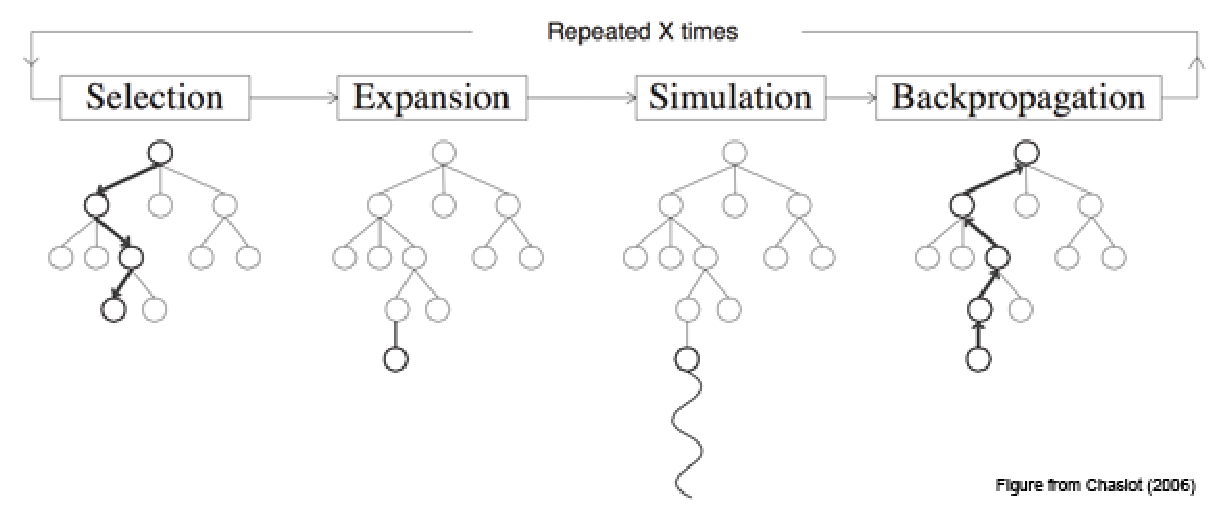
\includegraphics[width=14cm]{img/mcts-algorithm-1a.eps}
\end{center}
\caption{\footnotesize Monte-Carlo Tree Search.}{\footnotesize Monte-Carlo tree search consists
of iterating over four phases and can be interrupted at any time. Figure originates from
\cite{ChaslotPhd2010}.}
\label{fig_mcts_loop}
\end{figure}



\section{Algorithm Description}
\label{sec_mcts_description}

\citeauthor{Chaslot2008} provides good description of the Monte-Carlo Tree Search algorithm in
\cite{Chaslot2008}. Variant of MCTS as well as the terminology used in this thesis are based mainly
on this paper. Related pseudocodes follows this specific variant.


\begin{algorithm}
\DontPrintSemicolon
\caption{$Select(tree)$     \label{alg_select}}
\tcc{algorithm selecting a node for running a playout}
\KwData{$tree$\ldots MCTS tree}
\KwResult{Leaf node chosen by the selection is returned. The selection is determined by a particular
$SelectionStep$.}
$curr\_node \leftarrow Root(tree)$\;
\While{$curr\_node \in T$}{
    $last\_node \leftarrow curr\_node$\;
    $curr\_node \leftarrow SelectionStep(curr\_node)$\;
}
\Return{$last\_node$}\;
\end{algorithm}


\begin{algorithm}
\DontPrintSemicolon
\caption{$Backpropagate(tree, node, rewards[\,])$
\label{alg_backpropagate}}
\tcc{simulation results propagation}
\KwData{$tree$ \ldots MCTS tree\\
$node$ \ldots node to which the rewards are being backpropagated\\
$rewards[\,]$ \ldots array of rewards }
\KwResult{$tree$ with playout rewards added to all $node$'s ascendants}
$AddRewards(node, rewards[\,])$\;
$parent \leftarrow Parent(node)$\;
\If{$parent \in tree$}{
    $Backpropagate(tree, parent, rewards[\,])$\;
}
\end{algorithm}

\begin{algorithm}
\DontPrintSemicolon
\caption{$MCTSLoop(tree)$\label{alg_mcts}}
\tcc{main MCTS computation loop}
\KwData{$tree$\ldots MCTS tree}
\KwResult{$tree$ is enlarged by newly expanded nodes and results of playouts performed are added.
Node representing the best evaluated position reachable by one action is returned}
\While(\tcp*[h]{Main MCTS loop}){$EnoughTime()$}{
    $node \leftarrow Select(tree)$ \tcp*[h]{Phase 1: Selection}\;
    $node \leftarrow Expand(node)$ \tcp*[h]{Phase 2: Expansion}\;
    $rewards[\,] \leftarrow Playouts(node)$ \tcp*[h]{Phase 3: Simulation}\;
    $Backpropagate(tree,node,rewards[\,])$ \tcp*[h]{Ph 4: Backpropagation}\;
}
\Return{$\argmax\limits_{n \in Children(root)}c_n$} \tcp*[h]{Return most visited child}\;
\end{algorithm}



Monte-Carlo Tree Search is iteratively building a search tree as depicted by Figure
\ref{fig_mcts_loop} (originally published in \cite{ChaslotPhd2010}) and Algorithms 
\ref{alg_select}, \ref{alg_backpropagate} and \ref{alg_mcts}
which follow the method in its generality. Further details of chosen variant of MCTS
are discussed in subsequent sections and their related Algorithms, namely \ref{alg_selection_step},
\ref{alg_expand}, \ref{alg_playouts} and \ref{alg_add_rewards}.

Each node $i$ of the tree $t$ contains at least two values - visit count $n_i$
saying how many random position evaluations have been performed from $i$ and all its
descendants and
actual value $v_i$ which aggregates the results of these evaluations (usually as an average).
In addition, the game position represented by $i$, $Position(i)$, and pointers defining
tree structure have to be included. 

Position $p$ represents the current game state. Following
functions are appliable to $p$: $Actions(p)$ returns set of actions performable in $p$,
$Step(p, a)$ returns new position reachable by performing action $a$ in $p$ and $Score(p) \in
[0;1]$ returns static evaluation of the position (e.g. current game score).

$Parent(i)$ is
pointing to the parent of the node or to the $NullNode$ if $i$ is the root of the tree.
$Children(i)$ is the set of $i$'s children nodes. Once $i$ is expanded, $Children(i)$ contains
nodes representing positions reachable by set of
distinct actions $Actions(p)$ performable from $p = Position(i)$.
Particular action required to reaching $i$'s child $j$ is $Action(j)$.

The
tree itself provides the pointer to its root $Root(t)$. Function $EnoughTime()$ returns $true$ if
there is enough time to pass at least one more MCTS iteration and return the best evaluated
node. We use also other notations in pseudocodes of our thesis which we omit to list here. All
such notations are at least covered by a comment in a pseudocode.

Each iteration of MCTS consists of four
phases - \emph{selection}, \emph{expansion}, \emph{simulation} and \emph{backpropagation}. During
the selection phase the 
algorithm passes through the tree to a particular leaf $i$ where better-evaluated but less-visited nodes
are preferred. Appropriate balance between these claims is main objective of this
phase. Once a leaf node is selected the expansion phase follows. In this phase, according to a
certan condition (which is usually condition on node's visit count), $i$ itself is selected, or
new nodes reachable by actions from $Actions(i)$ are added to set $Children(i)$ and any of these
nodes is selected.
The next phase, simulation (also called \emph{playout}), plays a random game (or several games) 
starting
in position defined by expanded node to the end (simulation may be possibly terminated earlier).
Results from the simulations are then backpropagated to all
expanded node's ancestors during the fourth phase - backpropagation. The phases of the MCTS and
their specific variants are
further discussed in subsequent sections.



\subsection{Selection}


The process of selection consists of selection steps passing from a node to one of its children.
Each such a step meets exploration-exploitation problem where exploitation tends to choose the
so far best evaluated node and exploration on the other side promotes
undiscovered ways in the tree. This problem can be viewed as instance of a well-known problem 
called the Multi-Armed Bandit Problem (MAB). Its definition is adopted from \cite{Auer2002} and 
\cite{Kocsis2006}:

\newtheorem*{defmab}{Definition}
\begin{defmab}[K-armed bandit problem] 

Let us have independent random variables $X_{i,n}$ for $1 \le i \le K$ and $n \ge 1$. Each $i$ is
the index of a gambling machine and $X_{i,1}$, $X_{i,2}$,\ldots are identically distributed rewards
with unknown expected value $\mu_i$ yielded by successive plays of machine $i$. For the simplicity
the rewards are bounded to $[0,1]$.

A \textbf{policy} $A$ is an algorithm that chooses the next machine to play based on the sequence of
past plays and obtained rewards. Let $n_i$ be the number of times machine $i$ has been played by
$A$ during the first $n$ plays and $I_i^A$ be the index of a machine played in nth play. Then the
regret of A after n plays is defined as

\begin{equation}
R_n^A = n \mu^* - \sum_{j=1}^K n_j \mu_j \mathrm{,\;where}\;\mu^* \stackrel{\mathrm{def}}{=}
\max_{1 \le i \le K} \mu_i
\end{equation}

thus the \textbf{regret} $R_n^A$ is the loss caused by the policy not always playing the best machine.

\textbf{K-armed bandit problem} consists in finding optimal policy $A^*$ minimizing
expected regret $R_n^A$.

\end{defmab}


\Citeauthor{Auer2002} introduced computationaly effective optimal policy UCB1 \cite{Auer2002} 
having regret bounded to $O(\log{n})$. Abbreviation UCB stands for \emph{Upper-Confidence Bound}
and refers to value maximized by the policy. Let us define the value of UCB1:

\begin{equation}
UCB1(\bar{X}_{i,n_i},n,n_i) = 
    \left\{
        \begin{array}{c@{\quad\quad}l}
            \bar{X}_{i,n_i} + \sqrt{{2 \log{n}} \over n_i} & if \quad n_i > 0 \\
            \infty & otherwise \\
        \end{array}
    \right.
\end{equation}.


Then the policy itself chooses the machine as follows:

\begin{equation}
 I_{UCB1}(n+1) = \argmax\limits_{i\in{1,\ldots,K}} UCB1(\bar{X}_{i,n_i},n,n_i)
 \end{equation}.

UCB1 consists of average of previous rewards and a bias decreasing with number of the
machine's plays. In addition significance of the bias is growing with the total number of plays
what
leads to increase of exploration. Each machine is tried once before further selection based on
previous evaluation and the bias is used. This is forced by setting UCB1 value to $\infty$ for
machines not yet tried.

UCB1 applied to Trees \cite{Kocsis2006} is specific selection stratedy we use in our thesis. It 
is derived from UCB1 using values $v_i$ and $n_i$ stored in
particular node $i$. In addition the bias coefficient C is introduced in \cite{Chaslot2008}.
The purpose of this coefficient is tuning the balance between exploration and exploitation.
UCB1 contains fixed value of $C$ equal to $\sqrt{2}$ which can be used as good reference value.
Tuning of $C$ is usually done 
experimentally. The form of the formula for UCT and related selection applied in node $p$ is as
follows:

\begin{align}
    &\begin{aligned}
UCT(v_i,n_p,n_i) &= \left\{
        \begin{array}{c@{\quad\quad}l}
            v_i + C \sqrt{{\log{n_p}} \over n_i} & if \quad n_i > 0 \\
            \infty & otherwise \\
        \end{array}
    \right.
    \end{aligned}\\
    &\begin{aligned}
I_{UCT}^p &= \argmax\limits_{i \in Children(j)} UCT(v_i, n_p, n_i)
    \end{aligned}
\end{align}



According to the UCT, the selection passes down through the tree starting in the
root where the child with greatest UCT value is chosen in each node until a leaf is reached.
As mentioned in \cite{Chaslot2008}, experimental results show that the UCT value does not 
guide the selection well until
enough trials have been performed in node $p$ ($n_p$ is too small). To overcome this empirical
finding, the selection is guided by \emph{simulation strategy} which uses domain-specific
information (described in section
\ref{sec_simulation}) until $n_p$ does not reach certain threshold T. Selection phase
consisting of selection steps is
depicted by Algorithm \ref{alg_select}. The selection steps using UCT selection strategy is 
then depicted by Algorithm
\ref{alg_selection_step}. In our implementation of MCTS, we use the UCT. In MCTS for a game 
of Go in \cite{Chaslot2008} the constants used are $C= 0.7$ and $T=30$.

\begin{algorithm}
\DontPrintSemicolon
\caption{$UCTSelectionStep(node)$
\label{alg_selection_step}}
\tcc{one step of selection phase, an unvisited child, or a child having best UCT of given node
is selected}
\KwData{$node$\ldots a node of MCTS tree}
\KwResult{a children node chosen by a selection}
\If(\tcp*[h]{$node$ is a leaf or terminal node}){$Children(node)=\varnothing$}{
    \Return{$NullNode$}
}
\If(\tcp*[h]{Not enough simulations played}){$n_{node} < T_s$}{
    \Return{$SimulationStep(node)$} \tcp*[h]{Follow simulation strategy}
}
\If{$\exists i \in Children(node)$ such that $n_i=0$}{
    \Return{$i$} \tcp*[h]{Try all children first}
}
\Return{$\argmax\limits_{i \in Children(node)} \left( v_i + C \sqrt{\log{n_{node}} \over n_i}
\right)$} \tcp*[h]{Follow UCT value}
\end{algorithm}



\subsection{Expansion}
\label{sec_expansion}


\begin{algorithm}
\DontPrintSemicolon
\caption{$Expand(node)$\label{alg_expand}}
\tcc{expansion of an unexpanded node}
\KwData{$node$\ldots a leaf node of MCTS tree}
\KwResult{$node$ itself is returned, or new children reachable by actions valid in position
defined by $node$ are added to
$node$. One if these children is then returned.}
\If(\tcp*[h]{Not enough simulations performed}){$n_{node} < T_e$}{
    \Return{$node$}
}
\If(\tcp*[h]{$node$ is a terminal node}){$Actions(node) = \varnothing$}{
    \Return{$node$}
}
\ForEach{$action \in Actions(node)$}{
    $next\_pos \leftarrow Step(Position(node), action)$\;
    $child \leftarrow new\;Node(next\_pos, action)$\;
    $Children(node) \leftarrow Children(node) \cup \{ child \}$\;
}
\Return{$child$}
\end{algorithm}

The expansion decides whether or not will be the selected leaf expanded and so if the simulation
will begin in the leaf itself or in one of its children. The most common variant used also in our
thesis is that the node is
expanded once it reaches a particular visit count $T_e$. Greater value in such a condition causes higher
simulation count in each node and so stronger evaluation. On the other hand the process of building
tree is slowed down. With $T_e=1$ the expansion becomes even simplier and the leaf is simply
expanded always. Algorithm \ref{alg_expand} ilustrates expansion performed after $T_e$
simulations have been performed from a leaf.


\subsection{Simulation}
\label{sec_simulation}

\begin{algorithm}
\DontPrintSemicolon
\caption{$Playouts(node)$
\label{alg_playouts}}
\tcc{simulation phase returning rewards from performed playouts}
\KwData{$node$\ldots a node of MCTS tree}
\KwResult{An array of results of performed simulations is returned.}
\For{$i\leftarrow 1$ \KwTo $SIMULATIONS\_COUNT$}{
    $p \leftarrow Position(node)$\;
    \While{$\mathbf{not}\;TerminalCondition(p)$}{
        $p \leftarrow Step(p, SimulationAction(p))$\;
    }
    $rewards[i] \leftarrow Score(p)$\;
}
\Return{$rewards[\,]$}
\end{algorithm}

The simulation, or \emph{playout}, performs random play starting in the position defined in the
node selected by previous phases - selection and expansion. Simulation steps can be plain
random actions or, to improve the strength of
simulation, the simulation can follow a pseudo-random \emph{simulation strategy} designed according to
domain-specific information. Proper compromise between random play and following deterministic
heuristic has to be chosen.

In original Monte-Carlo tree search, the simulation is terminated at the end of simulated game.
To spare time spent in simulations, we can also terminate it earlier on certain condition
\cite{Ikehata2011} (e.g. number of simulation can be limited). After the termination, player's
position score is returned (chosen, without loss of generality, from interval $[0;1]$).
Additionally, to speed up the simulation, the simulation steps can be performed in
simplified game environment.

Even if it is better to perform selection before each simulation to avoid multiple 
evaluations of weak positions, some cases requires running multiple simulations in this phase
(e.g. \emph{leaf parallelization} described in section \ref{sec_leaf_parallelization}). This is
the reason why the array of results is returned by $Playouts(node)$ depicted by Algorithm
\ref{alg_playouts} Number of simulations performed is denoted as $SIMULATIONS\_COUNT$, action
selected by simulation strategy in position $p$ as $SimulationAction(p)$ and terminal condition
as $TerminalCondition(p)$.


\subsection{Backpropagation}

The last phase of the MCTS iteration is the backpropagation. The task of this phase is to propagate
rewards provided by the simulation to all node's precedessors. Various backpropagation strategies
may be used, however, the plain average is crucial for good properties of UCT and performs
well in
practise. Hence the result set $rewards[\,]$ obtained by simulation is added to the node's value containing
average of simulations performed in its subtree which leads to the update formulae for
node $p$ used in Algorithm \ref{alg_add_rewards}.

\begin{algorithm}
\DontPrintSemicolon
\caption{$AddRewards(node,rewards[\,])$\label{alg_add_rewards}}
\tcc{adds backpropagated simulation results to node's value (average of al simulations) and
adjust visit count appropriately}
\KwData{$node$\ldots a node of MCTS tree\\$rewards[\,]$\ldots array of simulation rewards}
\KwResult{Simulation results $rewards[\,]$ are added to $node$'s value.}
$rlen \leftarrow Length(rewards[\,])$\;
$rsum \leftarrow \sum\limits_{i=1}^{rlen} rewards[i]$\;
$v_{node} \leftarrow {{v_{node} n_{node} + rsum}
    \over{n_{node} + rlen}}$\;
$n_{node} \leftarrow n_{node} + rlen$\;
\end{algorithm}


\subsection{Game Steps in the Tree}

In this section, we describe simple technique which we use. It provides repeated usage of
certain parts of MCTS tree in multiple game steps.

\begin{algorithm}
\DontPrintSemicolon
\caption{$MCTSGame()$\label{alg_mcts_game_step}}
\tcc{complete game play with MCTS player}
$game \leftarrow new\;Game$\;
$mctree \leftarrow new\;McTree(game) $\tcp*[h]{Empty tree rooted in new game position}\;
$P \leftarrow Player(this)$\tcp*[h]{our player}\;
\While{$game$ is not over}{
    $actions \leftarrow new\;ActionArray$ \tcp*[h]{empty map}\;
    \ForEach{opponent on turn $O$}{
        $actions[O] \leftarrow GetAction(O)$ \tcp*[h]{let opponent calculate turn}\;
    }
    $best \leftarrow MCTSLoop(mctree)$ \tcp*[h]{perform MCTS}\;
    $actions[P] \leftarrow Action(best)$\;
    $GameStep(game, actions)$\;
    \tcp*[h]{Replace $mctree$ with a subtree defined by $actions$}\;
    \ForEach{$player \in Keys(actions)$ ordered as in $mctree$}{
        $Root(mctree) \leftarrow Child(Root(mctree),actions[player])$\;
    }
}
\end{algorithm}

After the computation of the MCTS tree, the best action according to visit counts of root's
children is returned and underlying game object is updated by our action and actions of
opponents. After that, computation of new MCTS tree begins. Since we work with fully observable
environment, we know the action performed by opponents. In a tree built in previous game round
we have a node corresponding with the game object after the update so we don't need to build
the very new tree from a scratch and instead of that, we can use a subtree corresponding with
updated game object.

Since UCT selection leads to most promising nodes, it is highly probable
that actions played by opponents will lead to a subtree with high visit count (our action leads
to a subtree with highest visit count) and so we can use simulations of the subtree with a
benefit as shown by Algorithm \ref{alg_mcts_game_step} which depicts MCTS together with game
objects and opponents.


\section{Convergence of UCT for Two-Player Games}
\label{sec_minimax_convergence}

The UCT algorithm (as a variant of MCTS) has been suggested as converging to optimal solution for the
single-player games \cite{Kocsis2006}, the counter-example of the convergence for two-player
games with simultaneous moves has been proposed in \cite{Shafiei2009}. In order to make the
convergence to the optimal strategy possible in general, we
consider turn-based games (weak turn-based turn-based games with teams eventually) for the 
building of a MCTS tree using UCT
selection and for purposes of playing simultaneous games, we perform expansion of simultaneous
nodes described in Section \ref{sec_turn_based_game_conversion}.




\section{Parallel Monte-Carlo Tree Search}
\label{sec_parallel_mcts}

Our objective in this thesis is design of algorithms for distributed MCTS computation among
cooperative autonomous agents. Closest to such algorithms are works on parallelization of MCTS 
which are
strong inspiration for algorithms proposed in Chapter \ref{chap_dmcts_design}.

Several publications dealing with parallelization of Monte-Carlo Tree Search have been published
recently \cites{Cazenave2007}{Chaslot2008}{Teytaud2008}. Two kinds of the parallelization are
discussed in these papers - multi-core parallelization and cluster parallelization.

Multi-core parallelization refers to computation on a symmetric multiprocessor computer (SMP). In
this case memory is shared among all processor cores and and can be accessed with same
(generally low) latency by any core  and access to this memory is the same and low.
Access synchronization has to be managed using a mutex mechanism. Two techniques for
parallelization with no need for locking (\emph{leaf parallelization}, \emph{root parallelization},
\emph{simulation results passing}),
and two variants of parallelization with locking (\emph{tree parallelization}) have been proposed so
far. 

Cluster parallelization is more generalized approach to parallelization. Memory is not shared
between parallel processes and so the inter-process communication is realized by \emph{message
passing}. Latencies in inter-process communication have to be taken in consideration but on the
other hand no memory locking is necessary. Algorithms mentioned as not using memory locking in
previous paragraph are suitable also for cluster parallelization.

For the simplicity and due to fact that all algorithms can be used in multi-core environment, we 
use multi-core terminology in descriptions of algorithms, so parallel
computational flows will be referred as \emph{threads} and computational nodes as \emph{cores}.

Strength and speed measures for comparing of algorithms used in this section is described in
following section.

\subsection{Comparison Measures for Parallel MCTS Algorithms}
\label{sec_measures_parallel}

We will briefly describe measures used in comparisons of parallel MCTS algorithms described in
following sections. Strength-speedup measure is taken from \cite{Chaslot2008}. Other measures
described here are inspired by same article.

\emph{Strength} of a player choosing actions for playing a game $G$ against
opponents $O$ (for case of multi-player game) 
is expected value of player's score at the end of the game. For experimental evaluation of the
strength, finite set of games is played and average
\todo{std dev?}
 of scores obtained is used. For our
purposes the player is guided by MCTS-based algorithm. Its strength is dependent on time $T$
provided to the algorithm for computation. In case of parallel MCTS algorithms, each thread has
time $T$ for computation. Since parallel algorithms run in multiple threads, each having same
amount of time as plain MCTS, its strength should be greater than in case of plain MCTS and should 
grow with number $n$ of cores involved. For more ilustrative comparison of parallel algorithms,
we will use \emph{strength-speedup} measure. Let us consider parallel algorithm having time
$T_{par}$
for its running and its strength $S$. Plain MCTS needs time $T_{pl}$ to achieve same strength
$S$. Then strength-speedup is equal to ratio of $T_{pl} \over T_{par}$. In other words,
strength-speedup is the increase of time needed to achieve the same strength by plain MCTS.
For better comparison of parallel algorithms running on various numbers of threads, we will use 
the third measure, a ratio of strength-speedup to the number of cores available for parallel
algorithm, and call it \emph{strength-efficiency}. This ratio can be also seen as ratio between
resources needed by plain MCTS (only $T$) and parallel MCTS ($T$ multiplied by number of
cores).

Another measure appliable to MCTS is \emph{Simulations-per-Second}. It simply says how many
simulations per second is being performed. Analogically to strength measures,
\emph{Simulations-per-Second speedup} and \emph{Simulations-per-Second efficiency} are defined
as ratio of Simulations-per-Second of plain MCTS and parallel MCTS and same ratio divided by
number of cores. 


\subsection{Leaf Parallelization}
\label{sec_leaf_parallelization}

\begin{algorithm}
\DontPrintSemicolon
\caption{$LeafParallelizationPlayouts(node)$}
\label{alg_leaf_parallelization}
\tcc{simulation phase of leaf paralelization}
\KwData{$node$\ldots a node of MCTS tree}
\KwResult{Array of simulation resulults is returned}

$tree \leftarrow new\,McTree$ \tcp*[h]{Initialize empty tree}\;
$root \leftarrow Root(tree)$\;
\ForEach{available processor core $C$}{
    $thread\_count \leftarrow thread\_count + 1$\;
    $threads[thread\_count] \leftarrow new\,PlayoutThread$\;
    $Run(thread)$\;
}
\While(wait for simulations){$AnyThreadRunning(threads)$}{
    $Wait()$\;
}
\For{$i\leftarrow 1$ \KwTo $Length(threads[\,]$}{
    $rewards[i] \leftarrow Reward(threads[i])$\;
}
\Return{$rewards[\,]$}
\end{algorithm}

\emph{Leaf parallelization} is simple algorithm originally introduced in \cite{Cazenave2007} as
\emph{at-the-leaves parallelization}. Parallelization is used only during simulation phase where
multiple simulations are executed. 

Master thread traverses the root to the leaf according to selection strategy and expands selected
leaf at first. Then for each available processor core, one simulation is performed from position
defined by leaf. Master thread then waits until all simulations are finished and backpropagates
their results up through tree. Algorithm \ref{alg_leaf_parallelization} depicts simulation phase 
of leaf parallelization.

This approach is very easy to implement since no complicated synchronization is used
which is its main advantage. However, several disadvantages have to be mentioned. First, cores are
not fully loaded for two obvious reasons. Algorithm is single-threaded during selection, expansion
and backpropagation phases and so slave threads are sleeping. In addition, running time of
simulation threads differ due to their high unpredictability and threads which already finished
simulation have to wait for the last one. Second disadvantage is one that leaf parallelization
forces multiple simulations
per position. It leads to better position evaluation but slows the speed of tree building. Last
disadvantage is that in comparison with plain MCTS which performs selection after each simulation,
the leaf parallelization have to perform full set of simulations per each node and so some of
unnecessary simulations are uselessly performed because first few of them can serve as good evidence
for considering the position as a bad candidate for further exploration. This can be worked around
if simulation threads are terminated once such a consideration is made according to already finished
simulations.

Leaf parallelization is suitable for using in both multi-core and cluster environment.


\subsection{Root Parallelization}
\label{sec_root_parallelization}

\begin{algorithm}
\DontPrintSemicolon
\caption{$RootParallelizationMaster(random\_seed)$}
\label{alg_root_parallelization_master}
\tcc{master thread of root parallelization}
\KwData{$random\_seed$\ldots a random seed distincts from seeds of other threads}
\KwResult{Best action calculated by root parallelization alrogithm}

$tree \leftarrow new\,McTree$ \tcp*[h]{Initialize empty tree}\;
$MCTSLoop(tree)$ \tcp*[h]{Perform MCTS iterations}\;
$roots \leftarrow new\,RootSet$ \tcp*[h]{Empty set}\;
$roots \leftarrow roots \cup BuildNextActionTreeCut(tree)$ \tcp*[h]{Add own root}\;

\ForEach(\tcp*[h]{Receive roots}){Team-mate $P$}{
    $received\_root \leftarrow Receive(P)$\tcp*[h]{Wait for a root from $P$} \;
    $roots \leftarrow roots \cup received\_root$\;
}

\tcp*[h]{Merge roots} \;
$merged \leftarrow new\,McTree$ \;
\ForEach{$root \in roots$}{
    \ForEach{$leaf \in Leaves(root)$}{
        $node \leftarrow LookupNode(merged,Path(leaf))$ \tcp*[h]{new node is created if not found}\;
        $Backpropagate(merged,node,RewardsOf(leaf)$ \tcp*[h]{$leaf$ is merged into the tree} \;
    }
}

\Return{$\argmax\limits_{n \in Children(Root(merged))}c_n$} \tcp*[h]{Return most visited child}\;
\end{algorithm}

\begin{algorithm}
\DontPrintSemicolon
\caption{$RootParallelizationSlave(random\_seed,master\_thread)$}
\label{alg_root_parallelization_slave}
\tcc{slave threads of root parallelization}
\KwData{$random\_seed$\ldots a random seed distincts from seeds of other threads\\
$master\_thread$\ldots master thread}
\KwResult{Nothing. Best action is returned by master thread.}
$tree \leftarrow new\,McTree$ \tcp*[h]{Initialize empty tree}\;
$MCTSLoop(tree)$ \tcp*[h]{Perform MCTS iterations}\;
$root \leftarrow BuildNextActionTreeCut(tree)$ \tcp*[h]{Extract root}\;
$Send(master\_thread, Message(root))$\;
\end{algorithm}

Another approach first proposed in \cite{Cazenave2007} is \emph{root parallelization} being
originally named as \emph{single-run parallelization}. In root parallelization, independent
MCTS instance is executed for each core with different random-seeds so the trees built by individual
instances differ. Finally, roots with their children from all instances are collected in master
thread and merged. The result is set of nodes containing information from all MCTS instances which
are used for selecting the best action to perform. Main advantages are simple implementation and a
minimal amount of communication so root parallelization can be successfully used both in cluster
and multi-core environment.

The algorithm is ilustrated by Algorithms \ref{alg_root_parallelization_master} and 
\ref{alg_root_parallelization_slave} (1 master together with several slaves are run). 
In the algorithm, we use 
procedure $BuildNextActionTreeCut$ for extraction of tree root. Description of the procedure
and related pseudocode can be found in Section \ref{sec_root_exchanging_agents}.

There is a disadvantage resulting from missing communication during running of MCTS
instances. Because each MCTS tree is built separately each instance have to perform similar
exploration or in other words same set of positions have to be evaluated before interesting
positions can be inspected. Due to this disadvantage plain MCTS having proportionally more time for
running would still probably perform better because no duplicit exploration have to be done and such
a saved time can be used for deeper exploitation. However, according to comparisons resumed
in Section \ref{sec_parallel_mcts_comparison}, the root parallelization performs, at least for the 
game of Go, approximately equally to plain MCTS having adequately more time for computations
(time used by root parallelization algorithm times number of processors used).



\subsection{Tree Parallelization}

\todo{pseudocode?}

The reasons why leaf parallelization wastes too much time leaving cores in sleep are removed by
\emph{tree parallelization}. It is done by effective tree locking so individual threads can access
and modify the tree on their own and so particular simulations follow independent selections and
need not to wait for the end of other simulations. The tree can be locked with \emph{global mutex}
or with \emph{local mutexes} placed in all nodes. The global mutex is simplier method saving costs
associated with locking but the maximum speedup is significantly reduced because the average
percentage of time spent in the tree (denoted as $x$ for now) is usually relatively high ($25\%-50\%$) 
and
so it is not possible to reach speedup higher than $100/x$. This is because if each of $n$
threads is
accessing the tree exclusively and no one have to sleep, percentage of time spent in 
tree is
equal to $n x$ and so $n \le \lfloor {100 \over{x}} \rfloor$. Due to this limitation, local mutexes
are necessary for systems with greater number of cores. To beat the fact of high costs of locking and
unlocking, fast-access mutexes should be used (i.e. spinlocks).

One more disadvantage of root parallelization should be handled. Tree parallelization may, at
one time, run multiple evaluations of a single node in situation when firstly finished
simulations would mark a node with bad value and so other evaluations are not necessary. To
beat such behaviour, \emph{virtual loss} is added to the value of nodes traversed by selection
of each thread and then removed during backpropagation phase. Virtual loss suppresses multiple
simulations on single node in case of weak actual value but for promising positions, more than
one simulation can be performed at a time.



\subsection{Simulation Results Passing}
\label{sec_simulation_passing}

\begin{algorithm}
\DontPrintSemicolon
\caption{$SimulationResultsPassingLoop(tree)$}
\label{alg_simulation_results_passing}
\tcc{a thread of simulation results passing algorithm}
\KwData{$tree$ \ldots MCTS tree}
\KwResult{$tree$ is enlarged by calculated and received simulations}

\While(\tcp*[h]{Main MCTS loop}){$EnoughTime()$}{
    \While(\tcp*[h]{Receive messages}){receiving queue $Q$ not empty}{
        $(path,rewards[\,]) \leftarrow Pop(Q)$ \;
        $node \leftarrow LookupNode(tree,path)$ \tcp*[h]{new node is created if not found}\;
        $Backpropagate(tree,node,rewards)$ \;
    }
    $node \leftarrow Select(tree)$\;
    $node \leftarrow Expand(node)$\;
    $rewards[\,] \leftarrow Playouts(node)$\;
    $Backpropagate(tree,node,rewards[\,])$ \;
    \ForEach(\tcp*[h]{Send messages}){Team-mate $P$}{
        $SendSimulationResult(P, Message(Path(node),rewards[\,]))$ \;
    }
}

\Return{$\argmax\limits_{n \in Children(root)}c_n$} \tcp*[h]{Return most visited child}\;
\end{algorithm}



\emph{Simulation results passing} can be viewed as a trial of adaptation of \emph{tree
parallelization} to cluster environment. These two algorithms share the property of high amount of
communication which is naturally bigger problem in distributed environment.

Unlike tree parallelization, the simulation results passing is building search tree separately in
each thread and synchronizes these trees by broadcasting messages containing identification of
expanded node and resulting value of performed simulation. This value is then backpropagated in
trees of receiving threads. Master thread finally returns best action according to its tree.
Simulation results passing is depicted by Algorithm \ref{alg_simulation_results_passing}.

This algorithm relies on high throughput of the cluster environment. Requirements on the throughput
grows with number of parallel threads so algorithm is not suitable for massive parallelism. The
algorithm is designed for usage in cluster environment but can be of course used also in multi-core
environment.


\subsection{Comparison and Conclusion}
\label{sec_parallel_mcts_comparison}

We have sumarized known algorithms for parallelization of MCTS in both multi-core and cluster
environment. Three of them (leaf parallelization, root parallelization and tree
parallelization)
have been experimentally evaluated in \cite{Chaslot2008} in context of playing Go in multi-core
environment. For this purpose the \emph{strength speedup} measure has been used. It is equal to
 the ratio of time needed for plain
MCTS to reach the same strength. Brief summary of results is covered by Table
\ref{tab_parallel_mcts_comparison} and Figure \ref{fig_parallel_mcts_comparison}. The winner of comparison is root parallelization performing even
better than single-threaded MCTS in case of 2 and 4 parallel threads. This is interpreted as 
parallel MCTS algorithms with different random seeds exploit different local optima so better one
can be finally chosen. Second best performance showed tree parallelization using virtual loss. Other
algorithms performed very poorly especially in case of higher number of threads.

\begin{figure}
\begin{center}
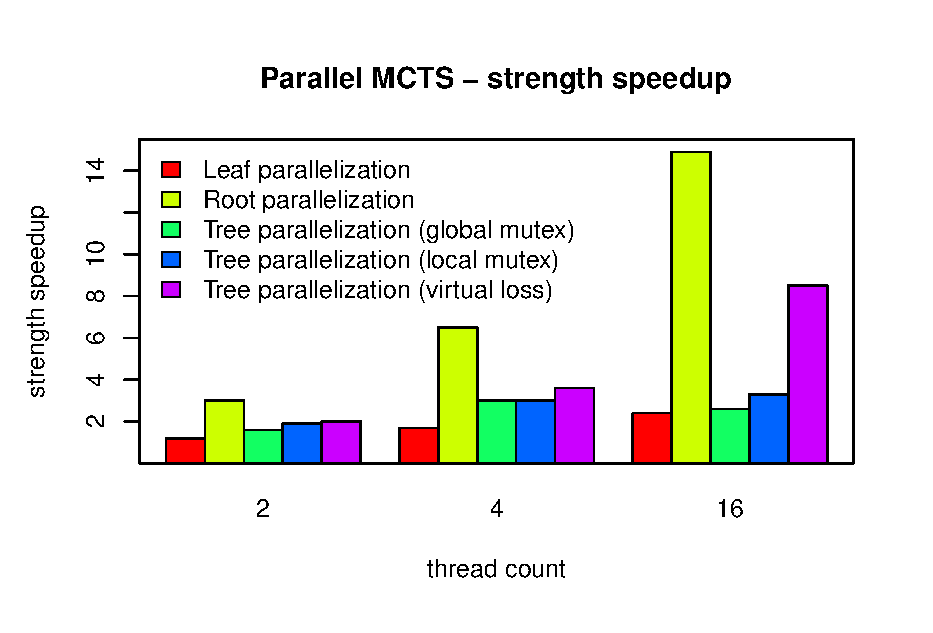
\includegraphics{img/parallel-mcts.eps}
\end{center}
\caption{\footnotesize Parallel MCTS algorithms - comparison.}{\footnotesize Strength-speedup
of parallel MCTS algorithms experimentally evaluated on Ms Pac-Man game in \cite{Chaslot2008}}
\label{fig_parallel_mcts_comparison}
\end{figure}

\begin{table}[h]
\label{tab_parallel_mcts_comparison}
\begin{center}
\begin{tabular}{|l|rrr|}
\hline Algorithm & 2 threads & 4 threads & 16 threads\\
\hline Leaf parallelization & 1.2 & 1.7 & 2.4\\
\hline Root parallelization & 3.0 & 6.5 & 14.9\\
\hline Tree parallelization (global mutex) & 1.6 & 3.0 & 2.6\\
\hline Tree parallelization (local mutex) & 1.9 & 3.0 & 3.3\\
\hline Tree parallelization (virtual loss) & 2.0 & 3.6 & 8.5\\
\hline
\end{tabular}
\end{center}
\caption{\footnotesize Parallel MCTS algorithms - comparison.}{\footnotesize Strength-speedup
of paralel MCTS algorithms experimentally evaluated on Ms Pac-Man game in \cite{Chaslot2008}}
\end{table}

%\begin{table}[h]
%\begin{center}
%\begin{tabular}{lrr}
%\hline
%Algorithm & Thread count & Strength speedup\\
%\hline
%Leaf parallelization & 2  & 1.2\\
%Leaf parallelization & 4  & 1.7\\
%Leaf parallelization & 16 & 2.4\\
%\hline
%Root parallelization & 2  & 3.0\\
%Root parallelization & 4  & 6.5\\
%Root parallelization & 16 & 14.9\\
%\hline
%Tree parallelization (global mutex) & 2  & 1.6\\
%Tree parallelization (global mutex) & 4  & 3.0\\
%Tree parallelization (global mutex) & 16 & 2.6\\
%\hline
%Tree parallelization (local mutex) & 2  & 1.9\\
%Tree parallelization (local mutex) & 4  & 3.0\\
%Tree parallelization (local mutex) & 16 & 3.3\\
%\hline
%Tree parallelization (virtual loss) & 2  & 2.0\\
%Tree parallelization (virtual loss) & 4  & 3.6\\
%Tree parallelization (virtual loss) & 16  & 8.5\\
%\hline
%\end{tabular}
%\end{center}
%\end{table}










\chapter{Distributed MCTS Algorithms for Cooperating Teams}
\label{chap_dmcts_design}



\section{Motivation and Problem Definition}

\todo{Upravit podle toho, co bude skutečně v kapitole \ref{chap_mas}}

We have already reviewed the Monte-Carlo Tree Search algorithm and its parallelization in
 Chapter \ref{chap_mcts} and distributed coordination algorithms in Chapter \ref{chap_mas}.
 The purpose of this chapter is design of distributed coordination algorithms based on
 Monte-Carlo Tree Search. Presented algorithms will work with MCTS tree kept indepentently in
 each cooperating agent. The tree will contain full information about actions done by all
 cooperating agents and also agents from opponent teams. This approach is supposed to be
 appropriate for games with small number of players but with increasing of the number of
 players, the branching factor grows and keeping full MCTS tree turns to be ineffective. The
 tree used in distributed algorithms along with general description of common parts of the
 algorithms are described in section \ref{sec_dmcts_common}. Before we will propose the
 algorithms description, it is necessary to introduce additional notations for this chapter in
 Section \ref{sec_notations_dmcts} and briefly discuss measures used for comparison of
 distributed algorithms in Section \ref{sec_measures_distributed}. \todo{Popis full MCTS stromu
 - zde nebo už v kapitole 1?}



\section{Useful Notations}
\label{sec_notations_dmcts}

In our algorithms, we will describe, among others, exchange of various parts of the MCTS trees of
the team-mates and it will be useful to give a formal definition of one of them, the so-called
\emph{tree cut}.

\newtheorem*{deftreecut}{Definition}
\begin{deftreecut}[Tree cut]

Let us have a tree $T$ with a set of nodes $N$. \textbf{Tree cut} $C_T$ is a subset of $N$ such that
there is no path between any ascendant $a$ of a node from $C_T$ and any descendant $d$ of a node from
$C_T$. In other words, nodes from a tree cut separates a subtree composed of nodes from $C_T$ and
their ascendants from the descendants of nodes from $C_T$. An example of a tree cut is depicted by
Figure \ref{fig_tree_cut_example}.

\begin{figure}
\begin{center}
\missingfigure{Tree Cut Example}
\end{center}
\caption{\footnotesize Tree Cut Example}{\footnotesize TODO}
\label{fig_tree_cut_example}
\end{figure}

\end{deftreecut}


\todo{Obrázek}



\section{Comparison Measures}
\label{sec_measures_distributed}

Measures suitable for plain Monte-Carlo Tree Search and parallel
Monte-Carlo Tree Search have been already described in Section \ref{sec_measures_parallel}.
We will show that these
measures are also suitable for comparison of distributed MCTS algorithms for games with team
of cooperating agents. In addition, we will compare the amount of communication needed by the
algorithms and the robustness of the algorithms against communication failures. For such
comparisons, we will evaluate strength measures depending on the amount of communication and
its robustness. The amount of communication will be simply the total length of messages
exchanged. Some environments (e.g. radio transmissions or Ethernet over coax) provide the 
possibility of broadcasting messages for the cost of passing single message whereas others 
don't so the cost of broadcasted message equals to the cost of separate messages to all
receivers. We will distinguish between these
environments since some of the algorithms advantage from cheap message broadcasting.

We have described two classes of measures for parallel MCTS, \emph{strength-} and
\emph{simulations-per second-}based measures. Former one works with score obtained at the end
of a game and latter one counts number of MCTS iterations handled per time unit. Details of
these measures are discussed in Section \ref{sec_measures_parallel}. Obviously we can use
simulations-per-second measures, distribution is not obstacle, simulations are still performed
and these measures show the computational costs of distribution of computation. Similar is the
case of strength measures where the only difference is that agents decide the actions
independently but from outer point of view the joint action is the same as if plain or parallel
MCTS calculate action. Strength measures say how strong is team guided by an algorithm.



\section{Proposed Algorithms}

\todo{Algoritmy s plným stromem x algoritmy inspirované DCOPy...}


\subsection{Backbone of the Distributed Algorithms}
\label{sec_dmcts_common}

\begin{algorithm}
\DontPrintSemicolon
\caption{$DistributedMCTSLoop(tree)$\label{alg_dmcts_common}}
\KwData{$tree$\ldots MCTS tree}
\KwResult{$tree$ is enlarged by newly expanded nodes and results of playouts performed are
added. Additional actions are performed during message receiving.
Node representing the best evaluated position reachable by one action is returned}
$i \leftarrow 1$\;
\While(\tcp*[h]{Main MCTS loop}){$EnoughTime()$}{
    \If{$i = 0$}{
        $ReceiveMessages()$\;
    }
    $node \leftarrow Select(tree)$ \tcp*[h]{Phase 1: Selection}\;
    $node \leftarrow Expand(node)$ \tcp*[h]{Phase 2: Expansion}\;
    $rewards[\,] \leftarrow Playouts(node)$ \tcp*[h]{Phase 3: Simulation}\;
    $Backpropagate(tree,node,rewards[\,])$ \tcp*[h]{Ph 4: Backpropagation}\;
    \If{$i = 0$}{
        $SendMessages()$\;
    }
    $i \leftarrow (i + 1)\;\mathrm{mod}\;N_{it}$\;
}
\Return{$\argmax\limits_{n \in Children(root)}c_n$} \tcp*[h]{Return most visited child}\;
\end{algorithm}

MCTS-based agents will iteratively build MCTS tree exactly as plain MCTS algorithm does. In
addition, before certain set of MCTS iterations, the agent receives messages from its team-mates
and performs appropriate actions. Similarly after the set of MCTS iterations, the agent
broadcasts messages to the team-mates. The communicaton between agents is the point differencing
particular distributed algorithms. Algorithms can also differ in other details such as random
seed intialization. Following subsections describe particular distributed algorithms.


\subsection{Independent Agents}

\todo{Okomentovat, proč se algoritmy jmenují Agents}

We will first describe the algorithm which is supposed to be the weakest one since no
communication between agents is performed. It serves as lower bound on performance of the
algorithms. The only trick used for the algorithm is setting of the random seed for the
simulation. Because there si no communication between agents, it can easily happen that agents
discovers different local minima. To avoid such a behaviour, the random seed for all agents are
set to same value during agent initialization. And because the agents have equal time to
compute the answer, the size of trees at the end of computation will be similar (this may not
be true for agents with inequal computational strength). If we suppose that all agents
calculate exactly the same number of iterations, time proposed to the agents is $t$ and the 
number of agents is $N$, then the
strength of this algorithm is supposed to be equal to the plain MCTS algorithm with computation
time equal to $t \over N$. This is obvious since the size of the tree of such a plain MCTS
algorithm is equal to trees computed by the independent agents. The only difference is that
independent agents have to calcupate their trees $N$-times since no communication is allowed.

Advantage of the algoritmh is that no communication is needed so it is not affected by
unreliability of the communication network.



\subsection{Joint-Action Exchanging Agents}

Simple way how to synchronize the movement of the agents is exchanging of the messages
containing the information about the actual best joint-action (tuple of actions of all
cooperating agents). The joint-action exchanging agents uses such a synchronization. When it is
a time to decide which action should be played, simple voting is used. Each agent sumarizes
most recent joint-actions received from all team-mates and uses the most frequent one. For
situations when multiple joint-actions with same frequency occurs, ordering on agents is
defined action played by agent higher in the ordering is played. To improve advantages of the
algorithms, different random seeds are used for initialization of the agents and so possibly
different local minima are considered during voting phase.

Such a communication is very low-cost and so does not require wide network channel. Since the
actual best joint-action does not change after very often, we can send the message only when it
is changed to further reduce costs on channel and computations related to networking. For cases
when network is too slow to handle all joint-action messages, all unsent messages (except one
which is being already transmitted) are flushed and the recent one is enqueued.


\subsection{Root Exchanging Agents}
\label{sec_root_exchanging_agents}

Joint-action exchanging agents are voting for the best joint-move but the tree from which the
joint-move is calculated contains only simulations done by the winning agent. Root exchanging
agents increase the strength of chosen action by merging of strengths of all possible 
joint-actions calculated by
all agents and so resulting joint-move is based on results from trees of all team-mates. This
strategy is based on root parallelization algorithm described in Section
\ref{sec_root_parallelization}.

Since the results from trees are merged, we want to build different trees in each action, so 
random seeds
are initialized to different values for each agent. The term "root" in this case means set of
actions $Actions(r)$ playable from the root $r$ of the MCTS tree together with their visit
counts $n_i, i \in Children(r)$. After the root merging, all agents have almost identical
set of joint-action -- visit-count pairs (some differences may occur since not the most recent roots
may be received at time of merging). Joint-action with highest summed visit count is
selected (ordering on joint-actions is used when multiple joint-actions have same visit count).

In case of single-player game, previous description of algorithm works well but there is a little
difficulty when any opponent is considered because set $Children(r)$ may not be a set of actions of
our team. We can simply wait for opponents' turn and exchange our messages during the period
when our team is on turn but this approach has two weaknesses. The first one is that this
perios may be very short what may, along with unreliable networking channel, lead to no
exchanging performed at all. The second weakness is that such a period for message
exchanging may not be present at all in case of turn-based game converted from simultaneous
game if current state was created by splitting simultaneous turn (see Section 
\ref{sec_turn_based_game_conversion}). We resolve this situation by extending definition of the
root for turn-based games with multiple teams. 

For multi-player games, the algorithm will exchange \emph{Next-Action Tree Cut} of a player $P$
being on turn. The Next-Action Tree Cut is defined as follows:

\newtheorem*{defnextactiontreecut}{Definition}
\begin{defnextactiontreecut}[Next-Action Tree cut]
Let us have a tree cut $C_1$ composed of nodes in which player $P$ is on turn and which are the first
nodes occuring on the path from tree root to its leaves. For all ascendants $C_1$, any player
different from $P$ is on turn. Then, we will call a set of children of nodes from $C_1$, which
also composes a tree cut, a \textbf{Next-Action Tree Cut} for a player $P$.

Algorithm \ref{alg_next_action_tree_cut_construction} describes construction of Next-Action
Tree Cut.i \emph{Popsat slovně algoritmus}

\end{defnextactiontreecut}

\begin{algorithm}
\DontPrintSemicolon
\caption{$BuildNextActionTreeCut(tree, player)$\label{alg_next_action_tree_cut_construction}}
\KwData{$tree$ \ldots MCTS tree \\
$player$ \ldots player constructing }
\KwResult{Algorithm returns the Next-Action Tree Cut of $tree$ for a player $P$}
$cut \leftarrow \{Root(tree)\}$ \tcp*[h]{cut growing from root}\;
$next\_action\_cut \leftarrow \{\}$ \tcp*[h]{final next action cut}\;
\While{$cut \not= \{\}$}{
    \ForEach{$node \in cut$}{
        $cut \leftarrow cut \setminus \{node\}$\;
        \eIf{$OnTurn(node)=P$}{
            $next\_action\_cut \leftarrow next\_action\_cut \cup Children(node)$\;
        }{
            $cut \leftarrow cut \cup Children(node)$\;
        }
    }
}
\Return{$next\_action\_cut$}
\end{algorithm}

Next-Action Tree Cut is being sent as array containing pairs of visit counts of nodes and
corresponding paths to the nodes represented as list of actions leading to the nodes. For
single-player game case, this approach leads to exchange of set of joint-action -- visit-count
pairs of root's children, how described earlier.

There is another difficulty with exchanging of Next-Action Tree Cut which is that the size of
the cut may grow excessively with growing number of players playing simultaneously so this 
algorithm is not suitable for such games. This fact should be kept in mind
when appropriate algorithm for a particular game is being chosen. When reliable communication
between agents is guaranteed, it is possible to safely exchange the cuts only in turns when the
player is on turn (considering simultaneous nature of the game). In case of unreliable
communication, on the other hand, information contained in cuts from turns when the player is
not on turn can be used with benefit if no communication can be done during the player's turn.


\subsection{Simulation Results Exchanging Agents}

\emph{Simulation Results Exchanging Agents} directly follow the idea of Simulation Results
Passing algorithm described in \ref{simulation_passing}. Since Simulation Results Passing
algorithm is designed for cluster environment, we have to deal with two main differences in
distributed coordination environment which are agents' independent reasoning and limited
and potentially unreliable communication. 

The former difference is simply managed by abandoning
the idea of master thread and letting all agents to play a calculated action. The latter one,
limited communication, is more serious issue. We cannot transmit all simulation calculated is
the channel is too narrow and so we have to choose which of simulation results will be
transmitted. We will prioritize simulation results which are more recent because such results
carry information about the interesting path in the MCTS tree (in comparison with less recent
ones which also carry the interesting path but not so long).

Mechanism of prioritizing of more recent simulation results is realized by message buffer
where, in opposite of common message sending, new messages with simulation results are inserted
at the beginning of the buffer. Once the buffer is full, the least recent messages are thrown
away.


\subsection{Tree-Cut Exchanging Agents}

Root exchanging agents share the information from their MCTS trees by sending messages
containing as little information as possible what spares the capacity of communication
channels but trees contain only calculations done by a particular agent. In opposite,
simulation results exchanging agents share full information about all simulations and so
each particular MCTS tree contains simulations from all agents and if the channel is reliable
and wide enough, it contains full information calculated together by all agents and all
trees are same. This approach, in comparison with root exchanging agents, brings some
advantages and also some disadvantages. 

Main advantage is higher robustness against
communication failures longer than time available for computation of one game step. Since
simulation results are applied into team-mates' trees, they don't vanish after a game step and
not even after several steps. Thanks to UCT mechanism, most of simulations are performed in
subtree which is finally chosen and all these simulations can be used during calculations of
the next action. This is beneficial also if no communication failure occur.

Most serious disadvantage of simulation results passing agents is that it requires wide
communication channel and if it is not available, only a proportional amount of simulations are
exchanged. Second disadvantage is that each received simulation has to be backpropagated
through the tree which requires additional time for computation.

\emph{Tree-cut exchanging agents} algorithm tries to find a compromise between root exchanging 
and simulation results passing. It keeps the advantage of received simulation results stored
directly in MCTS trees but aggregates them adequately to fit the width of the communication
channel. As a side effect of this approach, less calculation with received simulation results
is required.

\todo{Nepsat v textu názvy zbytečně s velkými písmeny}

Root exchanging agents algorithm constructs and sends the next-action tree cut. Similarly the
tree-cut exchanging agents algorithm sends a \emph{visit count tree cut} having following
properties: entire tree cut can be transmitted during time of one game step and visit counts of
nodes of the tree cut are similar. To add robustness to the algorithm, size of the tree cut is
chosen to a value such that the tree cut can be transmitted multiple times during the
one step calculation. We will denote the ratio between the byte size of the tree cut and bytes
transmitted during a turn as $C_{red}$ (\emph{red} for redundancy).

Tree-cut exchanging ghosts use different way of transmission of the tree cut. Root exchanging
ghosts send entire tree cut in one message while tree-cut exchanging ghosts send the tree cut
node by node what again increases the robustness because if one message is lost, only a small
part of information is lost which can be received next time the tree cut is transmitted or it
is calculated afterwards by receiving agent because the visit count node to which the lost node 
would be
applied is lesser and so UCT mechanism will lead the selection to subtree below this node. Each
node of the tree cut is transmitted as the triplet of path leading to the node, its value and
the visit count.

We define the visit count tree cut by introducing pseudocode for its construction, Algorithm
\ref{alg_visit_count_tree_cut_construction}. Algorithm starts with a tree cut containing only
the root of the MCTS tree and iteratively selects the node with highest visit count and
replaces the node with its children. The algorithm ends when desired byte size of the tree cut
is reached.

\begin{algorithm}
\DontPrintSemicolon
\caption{$BuildVisitCountTreeCut(tree,byte\_size)$\label{alg_visit_count_tree_cut_construction}}
\KwData{$tree\ldots MCTS tree$\\
$byte\_size\ldots desired size of the tree cut in bytes$}
\KwResult{Visit count tree cut of a given tree possible to transmit using less than
$byte\_size$ bytes}
$cut \leftarrow \{Root(tree)\}$ \tcp*[h]{cut growing from root}\;
$curr\_byte\_size \leftarrow ByteSize(Root(tree))$\;
\While{$true$}{
    $most\_visited \leftarrow \argmax_{i \in cut} n_i$\;
    $children \leftarrow Children(most\_visited)$\;
    $curr\_byte\_size \leftarrow curr\_byte\_size + ByteSize(children)$\;
    \If{$curr\_byte\_size>byte\_size$}{
        \textbf{break}\;
    }
    $cut \leftarrow cut \setminus \{most\_visited\} \cup children$\;
}
\Return{$cut$}
\end{algorithm}

Algorithm \ref{alg_visit_count_tree_cut_construction} builds a visit count tree cut for a
particular tree. Since the tree is changing after each iteration of MCTS, the tree cut is also
changing. For the sake of simplicity, the tree cut is fixed once it is built except of visit
counts of the nodes of the cut. This can lead to situation when transmitted tree cut is not the
visit count tree cut anymore because later simulation can focus on new undiscovered paths in
the tree. This property is a payment for a simplicity of the construction.

Other difficulty of the construction of visit count tree cut during the MCTS tree construction
is that the tree may not have enough size. To face this, the tree cut is built progressively.
Tree cut is kept even if its maximum byte size is not yet reached and after each MCTS
iteration, the tree cut is enlarged if maximum size has not yet been reached and appropriate
node in the cut for the expansion exist. To increase the representativeness of expanded node,
the expansion is not expanded immediately when it has children in the tree but when it reaches
sufficient visit count, denoted as $C_cut$. Progressive visit count tree cut building is
depicted by algorithm \ref{alg_progressive_visit_count_tree_cut_construction}. Tree-cut
exchange algorithm itself depicts Algorithm \ref{alg_tree_cut_exchange}.

\todo{Popsat mechanismus "přepisování" řezů}
\todo{pseudocode}

\chapter{Evaluation of Distributed MCTS Algorithms}
\label{chap_evaluation}

\section{Ms Pac-Man vs Ghosts Framework}
\label{sec_pacman_vs_ghosts}

For the purposes of evaluation of algorithms proposed in Chapter \ref{chap_dmcts_design}, we
have chosen the Ms Pac-Man vs Ghosts Framework \cite{PacmanVsGhosts} which is easy-to-use
framework allowing implementation of players for well-known old game Pac-Man in Java. Here we
will extract basics of the game rules used in the framework and afterwards we will
describe modifications of the rules we have done and reasons for them.

\subsection{Game Rules}

Ms Pac-Man is a game played in a maze in which two sides compete, the Pac-Man and four ghosts.
There are pills everywhere in the maze and Pac-Mans purpuse is to gather all the pills, each
for 10 points. Once all the pills are eaten, the game continues in a next maze. To complicate
the life of Pac-Man, ghosts are moving around the maze pursuing the Pac-Man and trying to
minimize its score. If the Pac-Man is caught, it will lose one life and if has any life
remaining, starts again from its starting position. Pills remain eaten after the life loss.
Ghosts appear in so-called lair at the beginning of each round and after Pac-Man's life loss
from where they start after a several time (different for each ghost). Beside regular pills,
each maze contains four power pills which are awarded with 50 points and when eaten by Pac-Man,
ghosts become edible and twice slower for certain period of time. Pac-Man can eat ghosts during 
this period for
reward of 200 points for first eaten ghost and 400, 800 and 1600 points for other ghosts.
Eaten ghost starts in lair again. Exact rules of the Ms Pac-Man vs Ghosts game can be found on the project webpage. 

The game was
additionally modified for purposes of testing of our algorithms. 
Our goal isn't to create strong player for Ms Pacman vs Ghosts competition but we want to test
proposed coordination algorithms and for such purposes, simplier testing environment giving
clearer results suits better.
Biggest change of rules is
removing power pills from the mazes together with entire edible ghosts mechanism. Reason for
this decision is lowering the variance of results. When Pac-Man is pursuing edible ghosts,
there is big difference in score when it eats different number of ghosts. For the same reason
three more modifications have been done. Pac-Man has only one life, game ends after the first
maze is cleared and random ghosts' reversal is suppressed. Random ghosts' reversal is a rule of
original Ms Pac-Man game bringing stochasticity to the game. If the rule is on, there is a 0.15\% 
probability each tick of a game that all
ghosts accidentally change their direction. Original game has a limit on maximum length of each
round after which score for remaining pills is added to Pac-Man's score and game continues to
the next level. This limit is set to 2000 what we keep as a rule, so our simplified game ends
after at most 2000 ticks. Limiting the number of rounds played together with limit on game
length also lets us run more tests.
An example of a situation from the game without
power pills is depicted by Figure \ref{fig_pacman_framework}.

\begin{figure}
\begin{center}
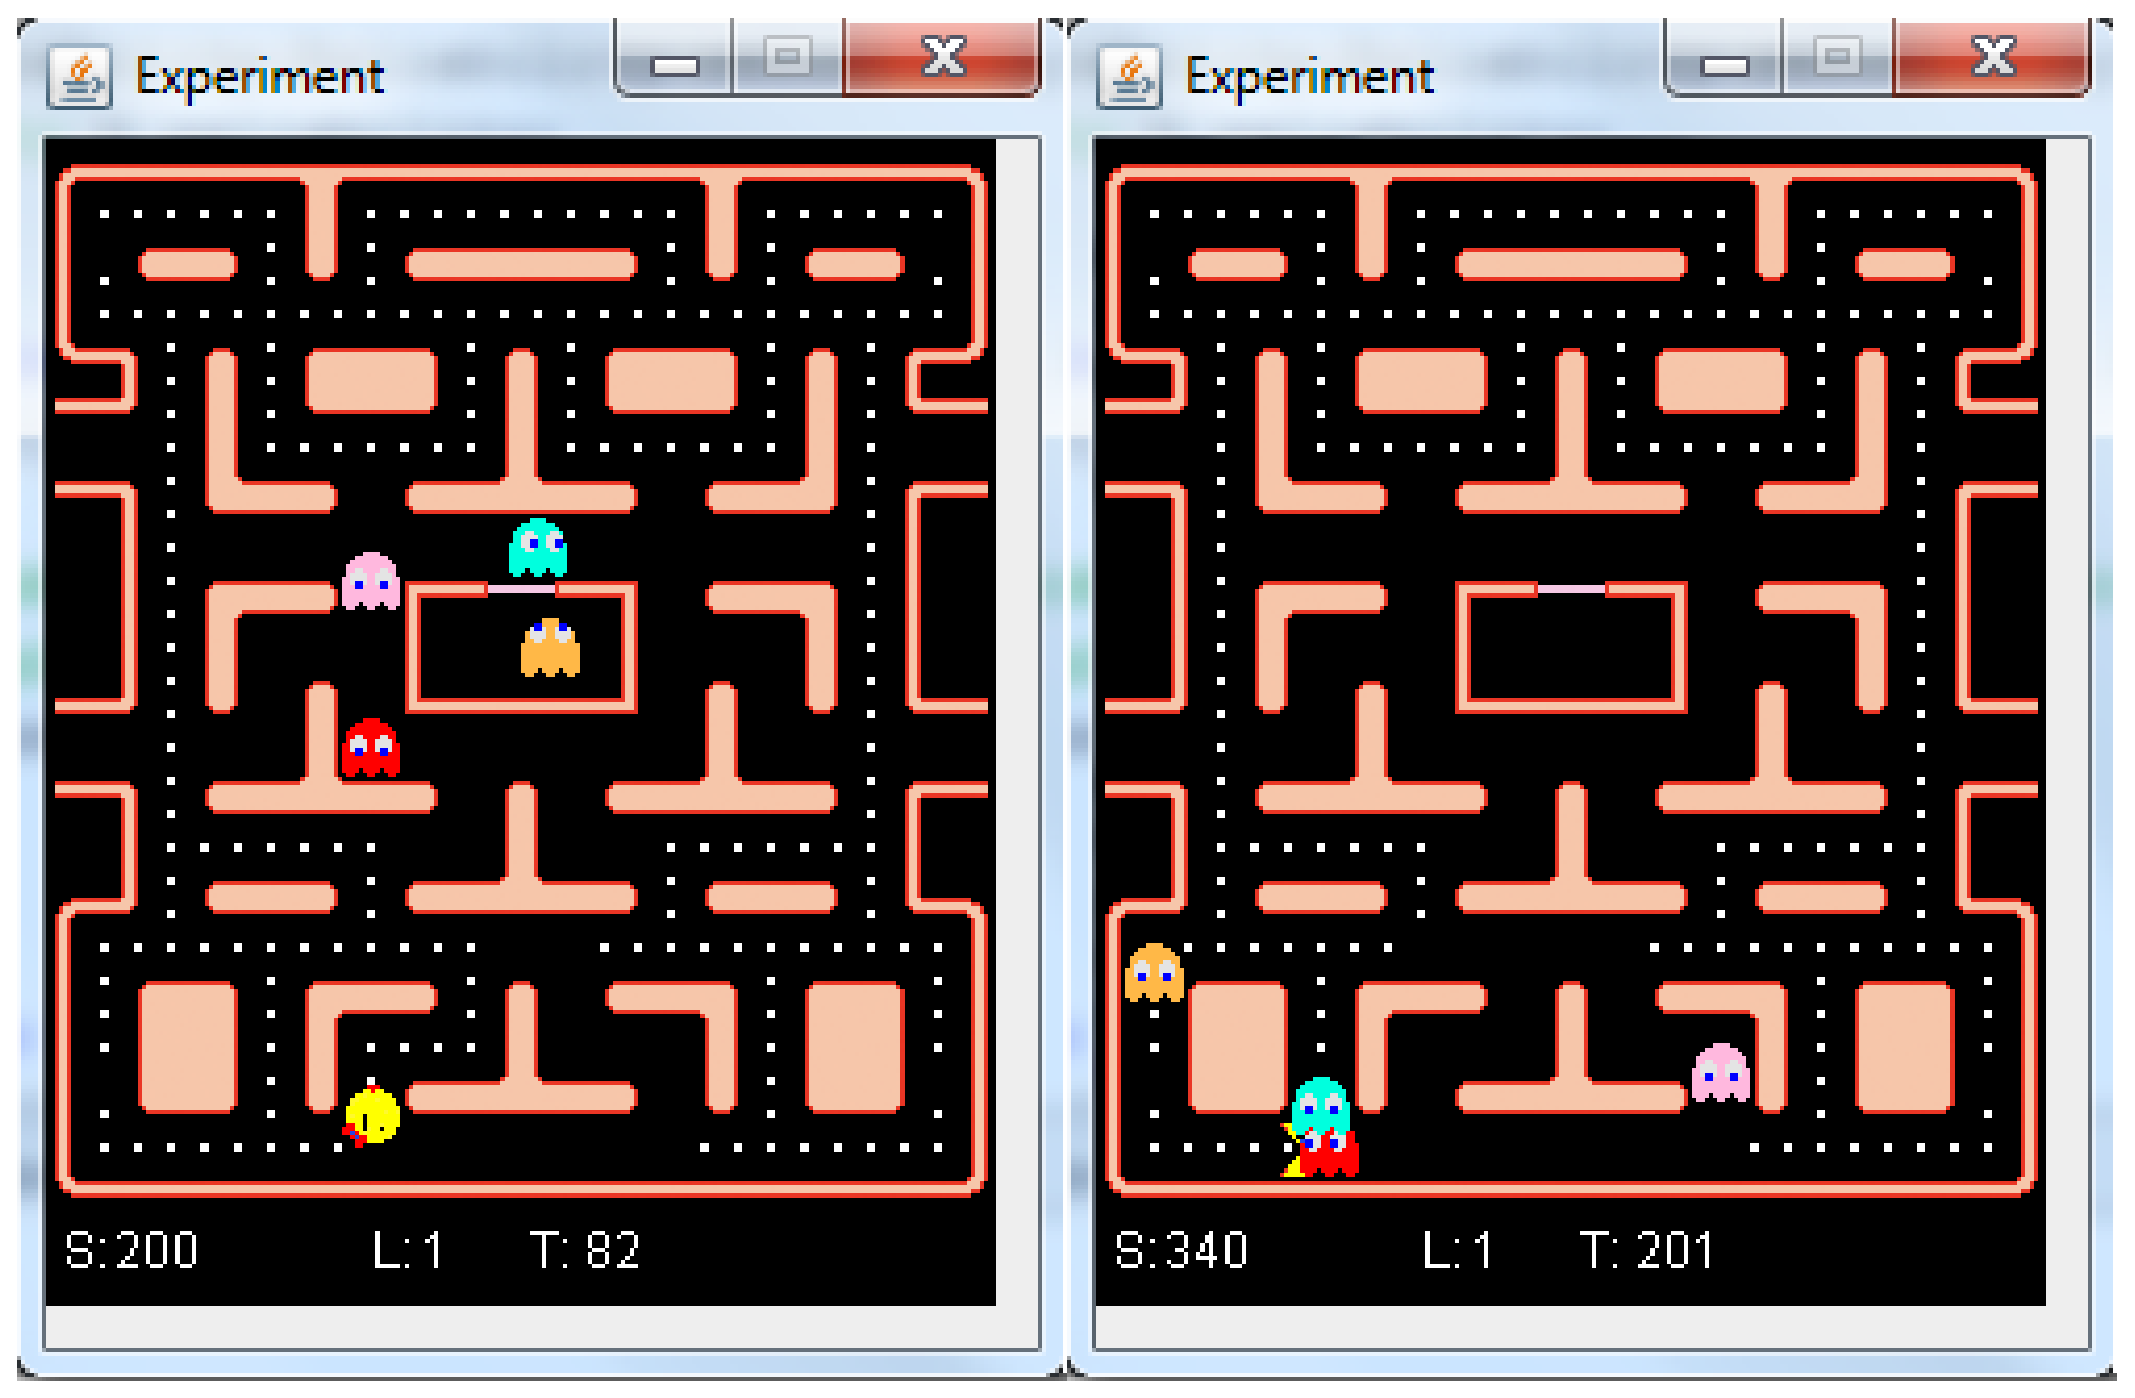
\includegraphics[width=14cm]{img/pacman_framework.eps}
\end{center}
\caption{\footnotesize Simplified game of Ms Pacman.}{\footnotesize Left picture shows the game few moments after it began. Three
ghosts started to hunt the Pac-Man while the orange one is still waiting in lair. Right
picture, on the other hand, shows the game just before the end. Pac-Man does not have any
escape path and is being caught with in a while with no life remaining.}
\label{fig_pacman_framework}
\end{figure}

Pac-Man has the same movement speed as non-edible ghosts. Paths inside the maze are divided
into small segments, four between two neighbouring pills. Pac-Man has to play an action after
at each segment, turning back in the middle of path or at the crossroad is allowed and so
Pac-Man has always at least two action to choose between. Contrarily, ghosts' movement is
restricted. Additional rule on ghosts' movement is that ghosts cannot turn back in the middle
of a path nor at a crossroad. That means that once a ghost chooses one way from a crossroad, it
has to continue to the end of the path. Despite of that, ghosts have to play an action on each
segment even though there is only one action to choose from.

So Pac-Man and ghosts play their actions at each segment of the maze but they, of course, have
to play an action in a limited time. Ms Pac-Man vs Ghosts framework provides by default 40 ms
to play what corresponds with the natural game timing when a human player controls Pac-Man.


\subsection{Framework Details}

In our thesis, we use Ms Ghost vs Pacman framework version 6.2. The framework is written in
Java what simplifies the development of controllers of the players. In original game, player
was able to control only Pac-Man and ghosts were controlled by simple AI. In the framework,
it is also possible to develop controller for the ghosts. The only work a user is supposed to 
do is
implement a controller of Pac-Man or ghosts, methods for running a game or a set of games are
prepared for usage. 

A player controller is a class implementing an interface having only one
method. In case of ghosts controller, method's header is \texttt{public EnumMap<GHOST,MOVE>
getMove(Game game,long timeDue)}, where \texttt{EnumMap<GHOST,MOVE>} is a joint-action of
ghosts, \texttt{game} contains information of current game and \texttt{timeDue} contains time
until which the method has to return an action.
If an action is not returned on time, certain
default action is chosen by framework itself.



\subsection{Pac-Man Opponents and Simple Ghosts Controllers}

To evaluate the strength of ghost controllers based on distributed MCTS algorithms, we need to
choose appropriate Pac-Man opponent to play against. Unfortunately, experiments with Pac-Man
controllers included in Ms Pacman vs Ghosts framework showed that these controllers are too
weak for evaluation. Thus, it was necessary to look for better Pac-Man controllers. 

Main purpose of the Ms Pacman vs Ghosts project is organizing competitions between existing
controllers. Competitions are usually held on various conferences and meanwhile there is also a
league  in which all controllers commited into the website compete. Thanks to the leagure
results we were able to contact authors of the league leading Pac-Man and obtained source code
of ICEP\_IDDFS \cite{IcepIddfs} what is controller based on iterative deepening depth-first
search approach. We haven't received more details about the controller. However, experiments
running against it have given promising results and so the controller was chosen as an opponent to
compare with.



\section{Implementation Notes}
\label{sec_implementation_notes}

In this section, we will discuss important implementation details of our controllers. As
mentioned in previous section, framework used for the experiments is written in Java and so
controllers are also supposed to be written in this language. We provide additional information
about software work in Attachment 2.


\subsection{Tree Construction}

Here we will talk about the way the concrete realization of MCTS tree for the game of Ms
Pac-Man. The most direct approach to a construction is to keep a node of the tree for each game
step and store, besides the value and the visit count, actions performed by Pac-Man and all
ghosts. By exposing and resolving of problems of this solution, we have reached the
construction used in our controllers.

First problem to be solved is that MCTS tree should not work with simultaneous actions of
multiple teams as discussed in Section \ref{sec_two_players_mcts}. 
Ms Pac-Man satisfies the definition of simultaneous game with teams, since multiple ghosts
together with Pac-Man may be on turn at a same time.
Section 
\ref{sec_turn_based_game_conversion} gives us a recipe to deal with simultaneous actions by
convertion of a simultaneous game to a (weak) turn-based game by splitting simultaneous nodes. The
conversion is not done on the unterlying Ms Pac-Man game itself but only for purposes of
expansion of nodes. When a simultaneous node is being expanded, instead of creating of a child
node for each pacman-ghosts joint-action, only children for each pacman action is created and
each of this children is immediately expanded with ghosts actions. By this approach,
simultaneous nodes are splitted according to optimistic expansion since in such a tree the
ghosts suppose to know the action of Pac-Man played in the simultaneous node. Our
implementation, in addition, supports the pesimistic expansion where ghosts actions are
expanded first in simultaneous nodes.

Second problem is quite high branching factor caused by Pac-Man which is able to change its
direction at any time. To reduce the branching factor, we consider additional rules of Pac-Man's
movement for purposes of node expansion. We allow Pac-Man to change its direction only at
crossroads, in the neighbourhood of a segment with not yet eaten power pill and at segments in
the middle of path when last segment allowing the direction change is exactly 6 segments far.
When computing the MCTS tree for Pac-Man, this reduction does not bring any difficulty since
the player controlled by the algorithm follows additional rules. But if we consider Pac-Man
playing against the MCTS algorithm, it may play an action not corresponding with these rules what
directly leads to desynchronization between game state and built tree. Next time any ghost
reaches  a crossroad and the desynchronization is detected, ghost play an action according to
the tree but then instead of using a subtree defined by the action for further computations,
new tree is built from scratch.

Finally, after expansion of simultaneous nodes and reduction of Pac-Man actions, the tree
will contain nodes having only one child which are also removed what adds a necessity to keep
lengths of edges between nodes.


\subsection{Pac-Man Playout}
\label{sec_impl_playout}

In our work, we decided to keep the simulation strategy simple, not leveraging much of
domain-specific information. This decision is driven by experiments from early phases of
development. During this experiments, both Pac-Man and ghosts players were, with a certain
probability, led by some heuristic algorithm inspired by original legacy behaviour in case of
ghost player and the StarterPacman example controller which is provided as a part of framework.
With supplementary probability, players performed random actions. Because we haven't discovered
any significant strength gain by tuning of the probability of heuristic steps, we omitted
heuristics at all.

The only additional knowledge put into the simulation strategy is that Pac-Man is not allowed
to change its direction in the middle of a path during simulation. The point of this 
restriction is that once Pac-Man enters a path, it usually wants to continue to a next
crossroad. In addition, such a restriction heightens expected size of area visited by Pac-Man
because situations of Pac-Man idling in the middle of path are suppressed.

We also use maximum depth of simulations. Tuning of this parameter is described in Section
\ref{sec_mcts_tuning}.

Simulations have to be evaluated after they finish. At first, we decided to use following
simple formula:

\begin{equation}
    { score\;reached } \over { maximum\;reachable\;score }
\end{equation}

But after some experiments, we realized that the formula does not enough motivate ghosts to
hunt pacman so we decided to add a bonus if ghosts successfully catch Pac-Man:

\begin{equation}
    (1 - \alpha) {{ score\;reached } \over { maximum\;reachable\;score }}
        + \alpha 
    \left\{
        \begin{array}{c@{\quad\quad}l}
            1 & if pacman\;was\;eaten\\
            0 & otherwise\\
        \end{array}
    \right.
\end{equation}

We call an $\alpha$ coefficient \emph{death\_weight} and tune it in Section
\ref{sec_mcts_tuning}.


\subsection{Communication}

Main method of a player controller (\texttt{getMove}) returns the joint-action
(\texttt{EnumMap<GHOST,MOVE>}) of the ghosts
but for purposes of distributed approach, each ghost is supposed to reason individually 
returning its action. To fulfil this, four subcontrollers, returning single \texttt{MOVE}
actions are started in four separated threads and virtual bidirectional communication 
channels are created between each pair of subcontrollers.

Channels provide interfaces for both senders and receivers and work with real time. Channel
consists of queue of messages to be sent and queue of received messages. Messages from the
sending queue to the receiving queue are transmitted every time a method on a channel is
called. Amount of messages transmitted corresponds with time elapsed since last channel event
ending with nonempty sending queue.

For purposes of evaluation of robustness of distributed algorithms againts communication
failures, channels contain a reliability object which simulates a reliability of a channel.
After a transmission of each message, the object determine if the message is really transmitted
to the receiver or if a failure occured and the message has to be discarded. The aim of the
reliability object is to filter messages to reach a percentual amount of messages successfully
transmitted. For the simplicity, we don't consider length of messages, messages of various
length have same probability of transmission. To model the reliability object closer to real
world, we decided not to use simple approach of single probability of transmission. Instead of
that, we work with two states of the object, \emph{reliable} and \emph{unreliable}, each
having a probability of successful transmission and a probability of a state change. In
reliable state, most of messages are transmitted and, contrariwise, most of messages are thrown
away in unreliable state. Such an
object is modelled as simple hidden Markov model depicted by Figure \ref{fig_hmm_reliability}.

\begin{figure}
\begin{center}
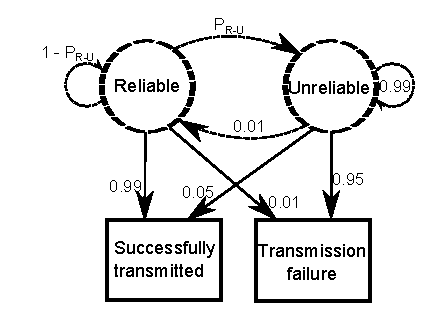
\includegraphics[width=8cm]{img/hmm_reliability.eps}
\end{center}
\caption{\footnotesize Communication reliability object.}{\footnotesize Communication 
reliability is modelled using hidden Markov model.}
\label{fig_hmm_reliability}
\end{figure}

We permanently set three parameters of a model - probability of transmission in reliable and
unreliable state and probability of transition from unreliable to reliable model, denoted as
$P_{R}$, $P_{U}$ and $P_{U\mhyphen R}$. Remaining
parameter, a probability of transmission from reliable to unreliable state, denoted as
$P_{R \mhyphen U}$, is calculated accordinly to desired percentage of time in reliable state
$Rel$.
Transittion between states is done every millisecond. Then expected length of a single period
of the object remaining in unreliable state is $\mathrm{E}P_U = {1 \over P_{U\mhyphen R}} \times 1
\mathrm{ms} = {1
\over 0.01}\,\mathrm{ms} = 100\,\mathrm{ms}$. Expected length of a reliable-state period is
$\mathrm{E}P_R = {1 \over
P_{R\mhyphen U}}$. $Rel$ is then equal to $\mathrm{E}P_R \over \mathrm{E}P_R + \mathrm{E}P_U$ and so 
$P_{R\mhyphen U}$ is
calculated from $Rel$ by the following equation.

\begin{equation}
P_{R\mhyphen U} = { 1 - Rel \over Rel } P_{R\mhyphen U}
\end{equation}

In case of tests not considering a reliability, all messages are transmitted. For tests with
altering reliability, $Rel$ is set to value between $0$ and $1$ and appropriate $P_{R\mhyphen
U}$ is used in HMM model.



\section{Experiments Setup and Methodics}
\label{sec_methodics}

All experiments were performed in virtualized environment of CentOS release 6.3 (Final) having
assigned 12 CPUs and 16 GiB of memory. Underlying host server disposes of 2 Intel(R) Xeon(R) 
CPU E5-2630 0 @ 2.30GHz processors (6 cores/12 threads each) and total of 128 GiB of memory.
Beside of our testing server, a few other virtual servers were running on the host server with
a light consumption of resources but taking into account that we were leveraging at most 4
cores at a time, remaining cores could easily handle the traffic. 


Java runtime used for experiments is \texttt{1.7.0\_09-icedtea}.

Simple bash scripts were used for purpuses of launching of individual games. Our Java
application contains uniform entry point allowing setting of necessary parameters for running
of an experiment. Each experiment were performed 100 times and average values were then used.
Data gathered during experiments were then processed in R environment. Graphs contained in this
work are also generated with R.


\section{MCTS Tuning}
\label{sec_mcts_tuning}

\begin{figure}
\begin{center}
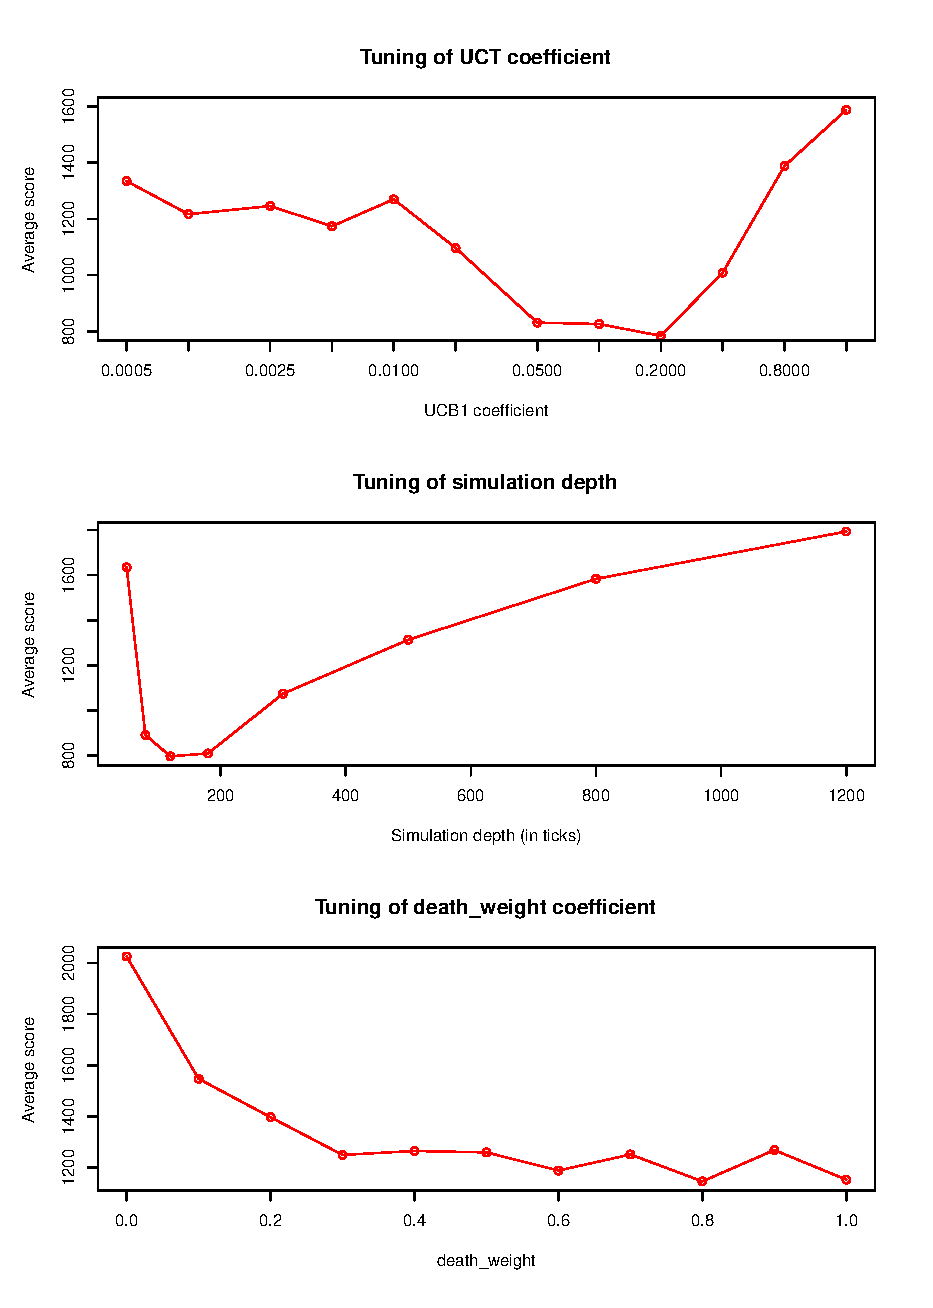
\includegraphics{img/mcts-tuning.eps}
\end{center}
\caption{\footnotesize Tuning of MCTS parameters.}{\footnotesize Top - tuning of UCT
coefficient, middle - tuning of maximum simulation depth, bottom - death\_weight tuning.}
\label{fig_mcts_tuning}
\end{figure}

Before we started any of our experiments, we wanted to be sure that our MCT alrogithm has
appropriate setting of parameters. We did three tests for approximate tuning of three
parameters - $C$ (UCT coefficient), simulation depth and \emph{death\_weight} (parameter used in
evaluation function, see Section \ref{sec_impl_playout}). Graphical results of these tests are
depicted by Figure \ref{fig_mcts_tuning}. All tunings were performed with a time ticks of 40
ms.

We first tuned $C$, with initial setting of simulation depth 200 and death weight 0.25. Test
showed us significant improvements with $C$ between 0.05 and 0.2 so we decided to use $C=0.1$.

Secondly, we tuned maximum depth of simulations, with already tuned $C=0.1$ and initial
$death\_weight=0.25$. According to the test, we set simulation depth to 120.

Finally, we tuned $death\_weight$ parameter used in evaluation formula with already tuned MCTS
parameters $C$ and simulation depth. According to the test, best values of the parameter are
between 0.3 and 1.0. During the evaluation of the test, some experiments with
$death\_weight=0.25$ were performing and a score with this $death\_weight$ didn't differ much,
we decided not to repeat the experiment with better setting of the parameter and run all tests
with $death\_weight=0.25$.



\section{Comparison of the Algorithms}
\label{sec_dmcts_experiments_comparison}

For distributed MCTS, three basic tests were performed. At first, strength of an algorithm
depending on computational time (length of single tick) with times from 10 ms to 200 ms, 100\%
reliable channel and channel speed fixed to a value of expected optimal communication
requirements. Second
test was strength in dependence on channel speed with fixed time set to 40 ms. Range of speeds
used depends on expected requirements on the communication so values
vary between tests. 
When we talk about average strength-speedup of some algorithm, we mean the average of
strength-speedups measuress for all measured computational times (10 ms-200 ms, stepping by 10
ms).
Channel speeds are scaled exponentially with values from $2^{lb}$ to
$2^{ub}$ for some algorithm-dependent values $lb,ub \in \mathbb{R}$.

We recall that the aim of the ghosts is minimization of Pac-Man's score so lower score indicates
better performance of the ghosts.

Next to the final score, we measured various other characteristics, such as average number of simulations
performed per second, average size of MCTS tree at moments requiring a decision or real ammount
of communication. These characteristics simplified analysis of behaviour of the algorithms.


\subsection{Centralized Monte-Carlo Tree Search}


\begin{figure}
\begin{center}
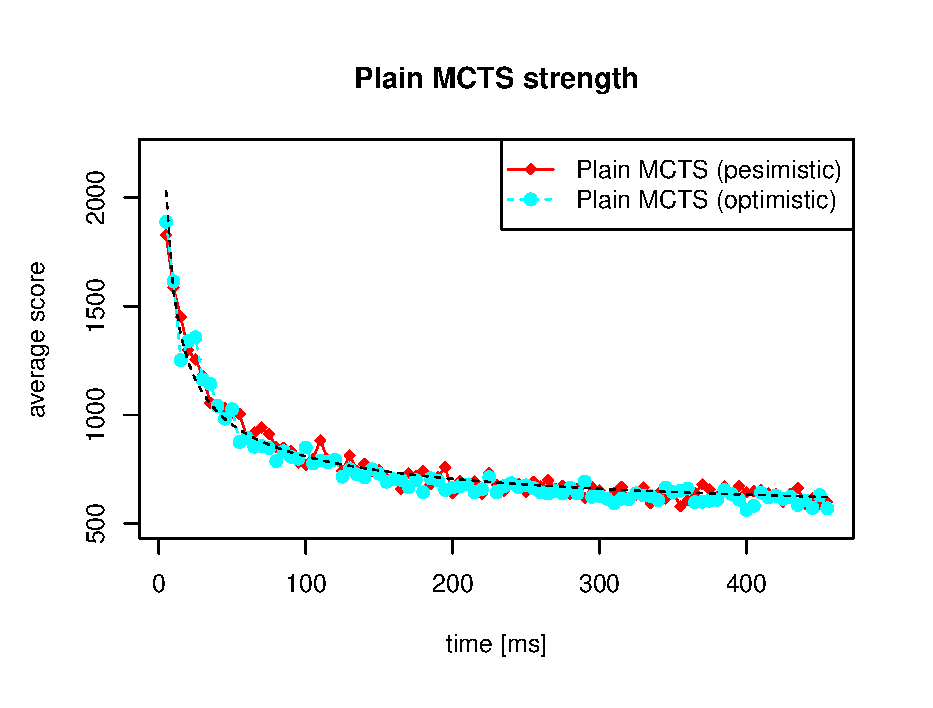
\includegraphics[width=14cm]{img/plain-mcts-strength.eps}
\end{center}
\caption{\footnotesize Plain MCTS strength.}{\footnotesize Red and green line shows strength 
of centralized MCTS with pesimistic and optimistic simultaneous nodes expansion. Dashed line is
a fit of data of red data to $c_0 + { c_1 \over \sqrt(t) }$. This fit is used for calculation
of strength-speedup of distributed algorithms.}
\label{fig_plain_mcts_strength}
\end{figure}


In Section \ref{sec_measures_distributed}, we defined the strength-speedup measure which
is used for comparison of distributed algorithms with plain (centralized) algorithm. So 
before we perform experiments with distributed algorithm, we run experiments with plain MCTS.
During these tests, we also compare approaches to expansion of simultaneous nodes in Ms Pac-Man
game. Average number of simulations calculated per second by plain MCTS algorithm was 11002.
This number will be also used for comparison of algorithm.

Figure \ref{fig_plain_mcts_strength} depicts results of plain MCTS running on single processor.
We tested both optimistic and pesimistic expansion of simultaneous nodes. Results haven't
showed a difference in performance of MCTS using these expansion. We have finally chosen
the pesimistic expansion for further experiments.

A shape of the curve connecting measured points in the figure does not follow decreasing
progression which is, of course, caused by measurement error and local minima overcame by the
convergence of MCTS. However, for purposes of the strength-speedup measure, we need to have
smooth and decreasing function of strength of plain MCTS. For the sake of the measure, we
calculate such a function by polynomial regression. We fitted measured data of plain MCTS with
pesimistic expansion on polynomial function $S(t) = c_0 + { c_1 \over \sqrt{t} }$, where $S$ stands
for strength (or score), $c_0,c_1$ are fitted
coefficients and $t$ is length of tick (time for computation). Form of $S(t)$ were suggested
according to shape of plotted data. The fitted function is drawn in
the figure as dashed curve. Once we know the regression of the plain MCTS strength, we can
simply calculate strength-speedup with usage of inverse function of $S(t)$.

\begin{equation}
%\begin{align}
%    &\begin{aligned}
        strength\mhyphen speedup(score, time) = {{ S^{-1}(score) } \over time }\\
        \end{equation}
        \begin{equation}
%    \end{aligned}\\
%    &\begin{aligned}
        \mathrm{where}\;\;S^{-1}(score) = {\left({c_1 \over {score - c_0}}\right)}^2
%    \end{aligned}
%\end{align}
\end{equation}



\subsection{Independent Agents}


\begin{figure}
\begin{center}
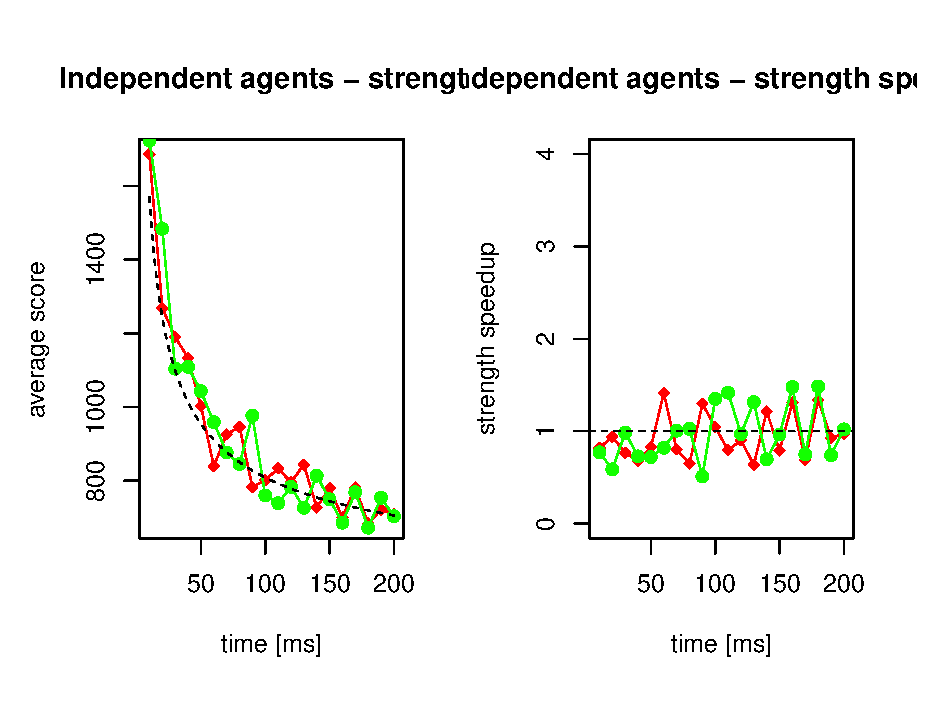
\includegraphics{img/dummy-ghosts-strength.eps}
\end{center}
\caption{\footnotesize Lorem ipsum}{\footnotesize }
\label{fig_independent_agents_strength}
\end{figure}

Independent agents does not perform any communication. Each of them build an independent MCTS
tree. The trees are synchronized by having same random seed for a construction of trees and so
trees are, after same number of interations, equal. For this algorithm, we expected strength
speedup approximately 1.0 or a bit lower (each agent usually manages to calculate slightly
different number of simulations what may lead to different calculated action and thus to
invalid synchronization).

For comparison, we tested also the independent agents algorithm with distinct random seeds.
Results are depicted by Figure \ref{fig_independent_agents_strength}. Average strength speedups
are 0.967 for equal random seeds and 0.941 for distinct random seeds what corresponds with
expectations.

Since there is no communication in algorithms, no further tests with altering communication
channel speed and channel reliability were done.


\subsection{Joint-Action Exchanging Agents}

\begin{figure}
\begin{center}
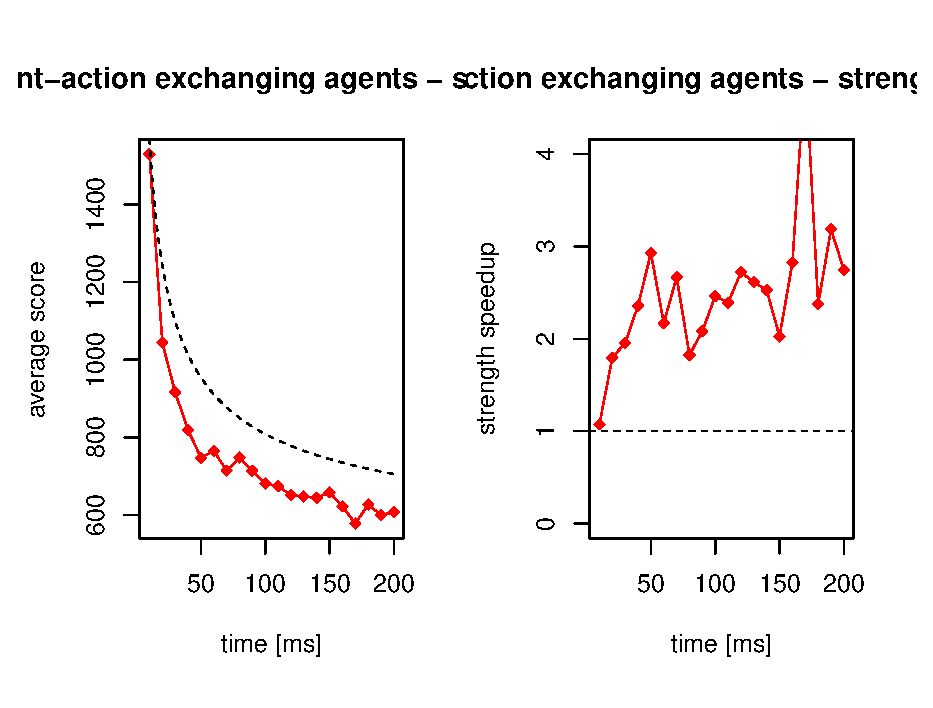
\includegraphics{img/move-exchange-strength.eps}
\end{center}
\caption{\footnotesize Lorem ipsum}{\footnotesize }
\label{fig_action_exchanging_strength}
\end{figure}

Joint-action exchanging agents serves for comparing more complex coordination methods with the
simplest imaginable one. Particular agents use only simulations calculated by themselves and
the only way how the algorithm can outperform plain MCTS is by choosing the best of local
minima calculated by agents. Surprisingly, the algorihm is quite successful and the mechanism
of voting for the best action reached a strength speedup of 1.73. This result overcame our
expectations.

\todo{Zavislost na sirce kanalu a reliability}


\subsection{Root Exchanging Agents}

\begin{figure}
\begin{center}
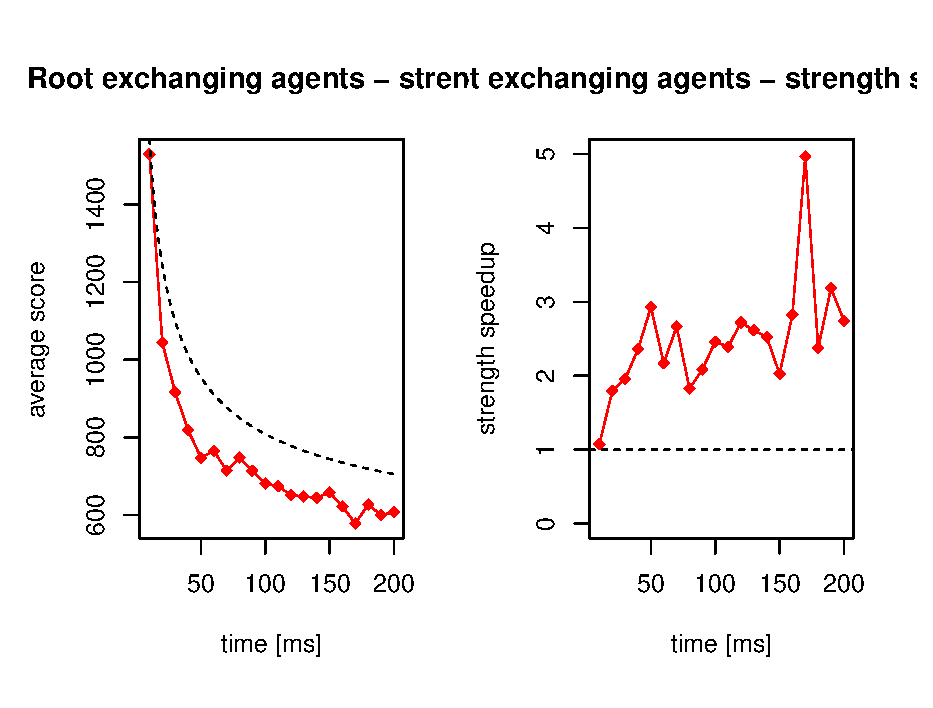
\includegraphics{img/root-exchange-strength.eps}
\end{center}
\caption{\footnotesize Lorem ipsum}{\footnotesize }
\label{fig_root_exchanging_strength}
\end{figure}

\todo{Vše přepočítat, uvést počet simulací za sekundu,...}

According to good results of root parallelization algorithm referred in Section
\ref{sec_parallel_mcts_comparison}, we expected good behaviour of an algorithm based on this
parallelization. Root exchanging agents reached average strength speedup 2.48 (average strength
efficiency 0.62)) 
what is below our
expectation. Root parallelization tests performed on a domain of the game of Go
\cite{Chaslot2008} showed results of strength efficiency around 1. The difference may be caused
by different game played. In both root parallelization and root exchanging agents algorithms,
each thread/agent computes own tree doing the same exploration of an empty tree. In opposite,
plain MCTS does only one exploration and so remaining computational time is used for deeper
exploration. The exploration is probably more important for Ms Pac-Man game and so the
disadvantage of shallower exploitation shows itself by lesser strength efficiency. Expenses of
handling of messages in our implementation is below 0.2\% of total time so \todo{!}



\begin{figure}
\begin{center}
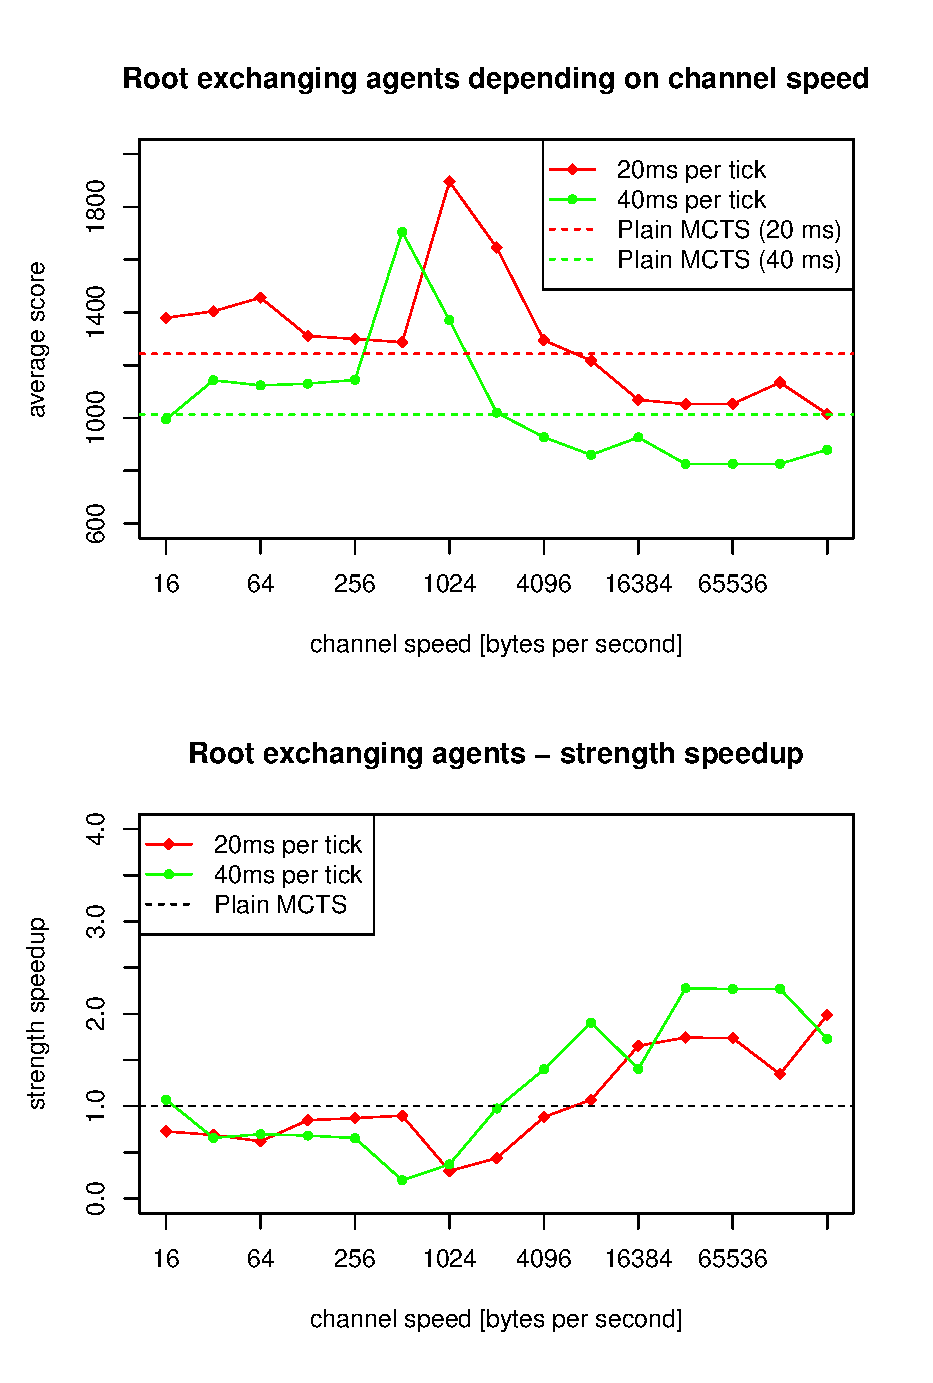
\includegraphics{img/root-exchange-channel-speed.eps}
\end{center}
\caption{\footnotesize Lorem ipsum}{\footnotesize }
\label{fig_root_exchanging_channel_speed}
\end{figure}




\subsection{Simulation Results Passing Agents}

The agents share full information about the performed simulations. In our implementation, the
ghosts need 256kB/s to reach a full performance of the algorithm, which is, expressed as
strength speedup, 1.60 in average. The algorithm performs worse than joint-action exchanging
agents. Expenses of such massive sharing among all trees are too high not only for requirements
on the width of communication channels but also for the amount of calculated simulations which
is reduced by approximately 1/3. Experimental results confirmed that this approach is robust
against communication failures. According to the experiments, the strength speedup remains
over 1.5 for the channel reliability 0.6 and higher. Results are ilustrated by Figures
\ref{fig_simulation_passing_strength}, \ref{fig_simulation_passing_channel_speed} and
\ref{fig_simulation_passing_unreliable}.


\begin{figure}
\begin{center}
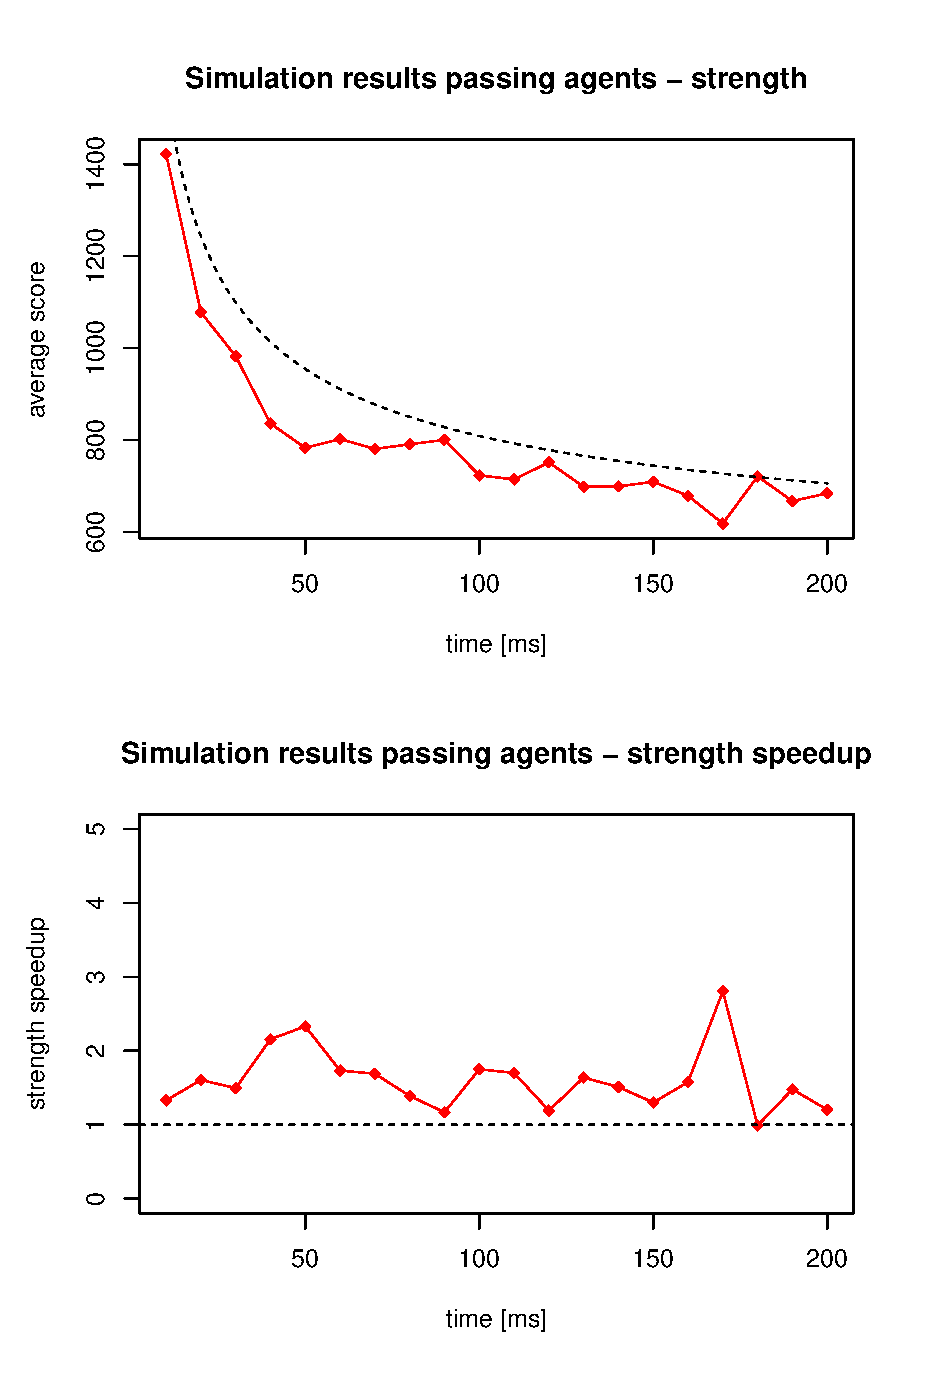
\includegraphics{img/simulation-passing-strength.eps}
\end{center}
\caption{\footnotesize Lorem ipsum}{\footnotesize }
\label{fig_simulation_passing_strength}
\end{figure}

\begin{figure}
\begin{center}
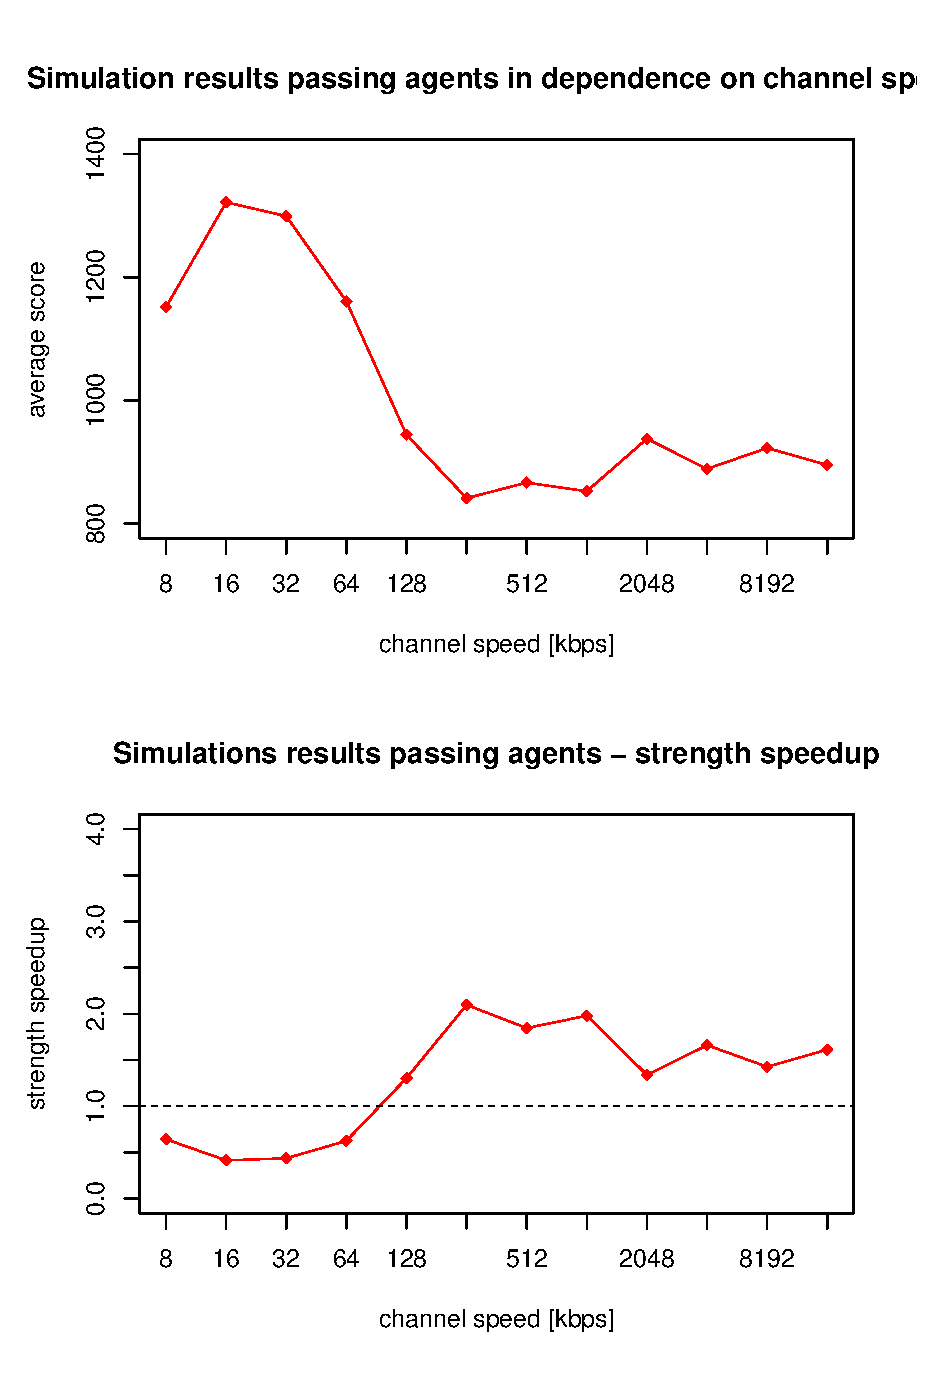
\includegraphics{img/simulation-passing-channel-speed.eps}
\end{center}
\caption{\footnotesize Lorem ipsum}{\footnotesize }
\label{fig_simulation_passing_channel_speed}
\end{figure}

\begin{figure}
\begin{center}
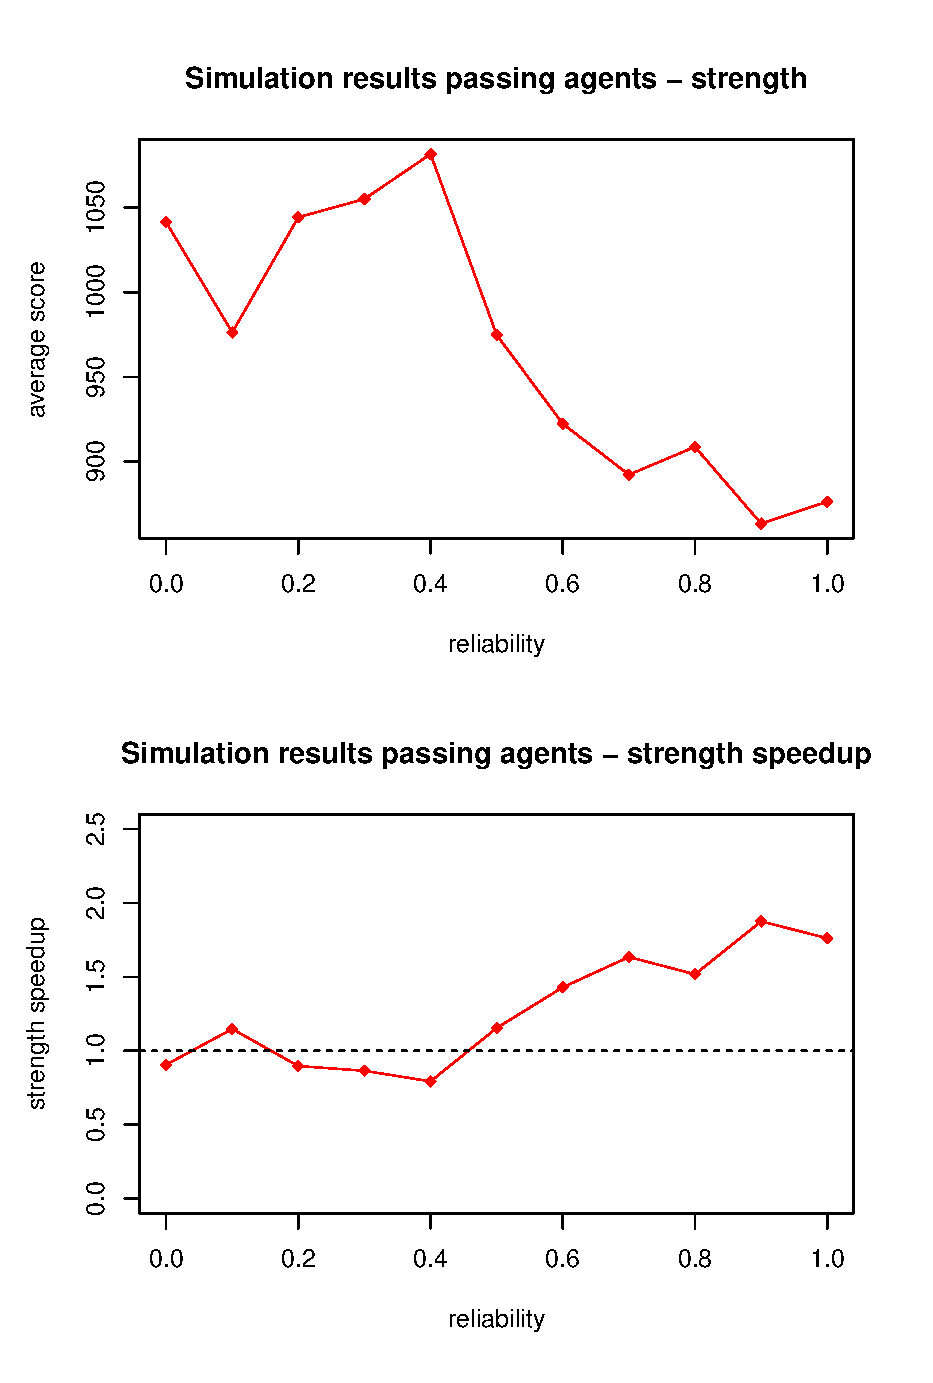
\includegraphics{img/simulation-passing-unreliable.eps}
\end{center}
\caption{\footnotesize Lorem ipsum}{\footnotesize }
\label{fig_simulation_passing_unreliable}
\end{figure}


\subsection{Tree-Cut Exchanging Agents}


\begin{figure}
\begin{center}
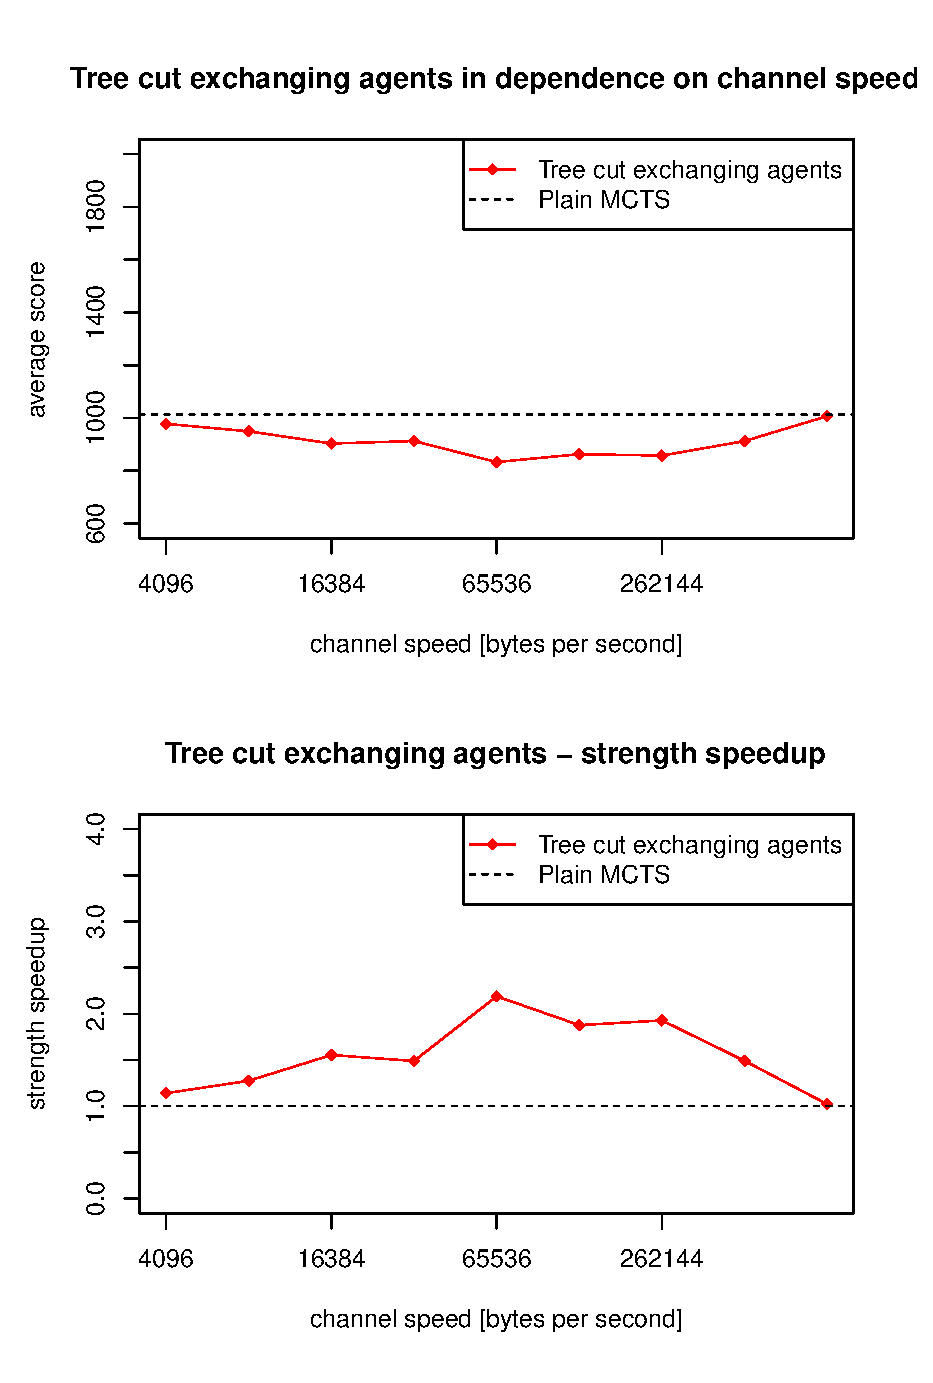
\includegraphics{img/tree-cut-channel-speed.eps}
\end{center}
\caption{\footnotesize Lorem ipsum}{\footnotesize }
\label{fig_tree_cut_channel_speed}
\end{figure}

\begin{figure}
\begin{center}
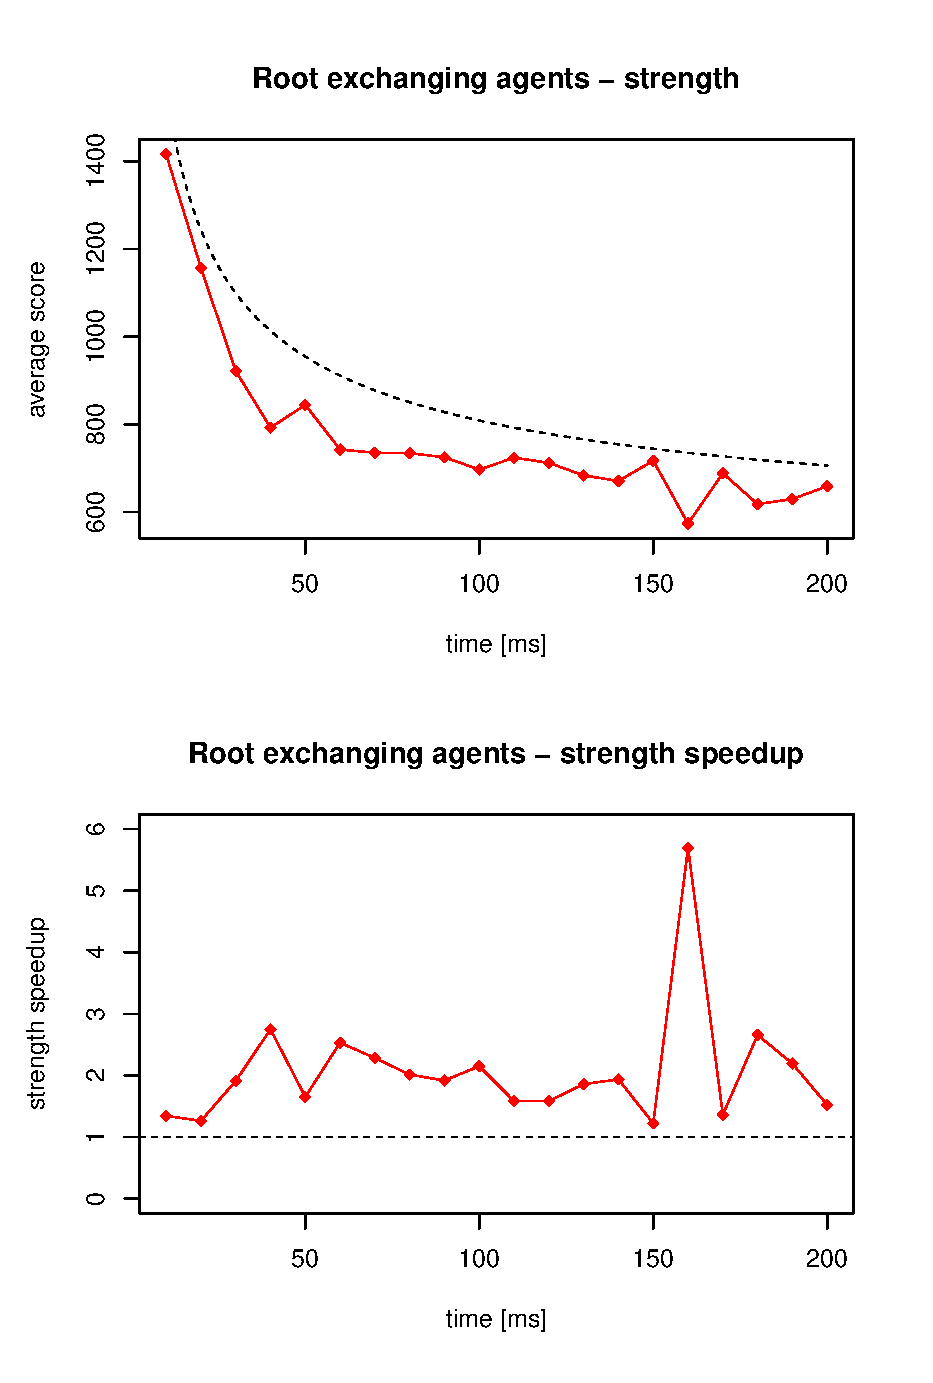
\includegraphics{img/tree-cut-strength.eps}
\end{center}
\caption{\footnotesize Lorem ipsum}{\footnotesize }
\label{fig_tree_cut_strength}
\end{figure}

\begin{figure}
\begin{center}
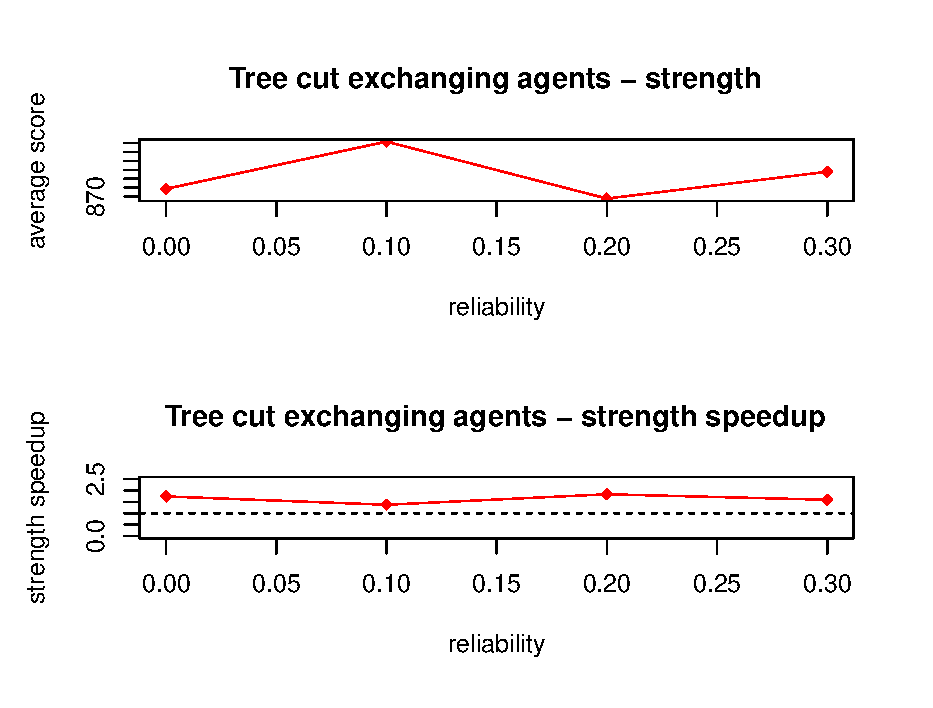
\includegraphics{img/tree-cut-unreliable.eps}
\end{center}
\caption{\footnotesize Lorem ipsum}{\footnotesize }
\label{fig_tree_cut_unreliable}
\end{figure}

\subsection{Comparison and Conclusion}

In Table \ref{tab_dmcts_comparison}, we provide synoptic comparison of the algorithms.
All algorithms have good robustness against communication failures. What differs is strength of
the algorithms (compared according to the results of the tests on Ms Pac-Man game) and
communication requirements. We consider root exchanging agents algorithm as the winner of
tests since it reached the best value of strength-speedup together with log requirements of
amount of communication.

\begin{table}[h]
\label{tab_dmcts_comparison}
\begin{tabular}{r|p{3cm}|p{3cm}|p{3cm}}
  & strength (speedup) & \parbox{3cm}{communication \\ requirements} & \parbox{3cm}{failure \\ robustness} \\
  \hline
  Independent agents & very bad (0.97) & no & - \\
  \hline
  Joint-action ex. ag. & bad (1.73) & very low & very good \\
  \hline
  Root ex. agents & good (..) & low & good \\
  \hline
  Sim. results passing ag. & bad (1.60) & very high & good \\
  \hline
  Tree-cut ex. agents & medium (2.07) & \parbox{3cm}{medium\\(scalable)} & \parbox{3cm}{good\\(scalable)} \\
  \hline
\end{tabular}
\caption{\footnotesize Lorem ipsum}{\footnotesize }
\end{table}


% Ukázka použití některých konstrukcí LateXu (odkomentujte, chcete-li)
% %%% Ukázka použití některých konstrukcí LaTeXu

\subsection{Ukázka \LaTeX{}u}
\label{ssec:ukazka}

This short subsection serves as an~example of basic \LaTeX{} constructs,
which can be useful for writing a~thesis.

Let us start with lists:

\begin{itemize}
\item The logo of Matfyz is displayed in figure~\ref{fig:mff}.
\item This is subsection~\ref{ssec:ukazka}.
\item Citing literature~\cite{lamport94}.
\end{itemize}

Different kinds of dashes:
red-black (short),
pages 16--22 (middle),
$45-44$ (minus),
and this is --- as you could have expected --- a~sentence-level dash,
which is the longest.
(Note that we have follwed \verb|a| by a~tilde instead of a~space
to avoid line breaks at that place.)

\newtheorem{theorem}{Theorem}
\newtheorem*{define}{Definition}	% Definice nečíslujeme, proto "*"

\begin{define}
A~{\sl Tree} is a connected graph with no cycles.
\end{define}

\begin{theorem}
This theorem is false.
\end{theorem}

\begin{proof}
False theorems do not have proofs.
\end{proof}

\begin{figure}
	\centering
	
\includegraphics[width=30mm]{../img/logo.eps}
	\caption{Logo of MFF UK}
	\label{fig:mff}
\end{figure}


\chapter*{Conclusion}
\section*{Summary}
\section*{Future Work}
\addcontentsline{toc}{chapter}{Conclusion}


%%% Seznam použité literatury
%%% Seznam použité literatury je zpracován podle platných standardů. Povinnou citační
%%% normou pro diplomovou práci je ISO 690. Jména časopisů lze uvádět zkráceně, ale jen
%%% v kodifikované podobě. Všechny použité zdroje a prameny musí být řádně citovány.
%
%def\bibname{Bibliography}
%begin{thebibliography}{99}
%addcontentsline{toc}{chapter}{\bibname}

%\bibliography{bibliography}
%\bibliography{plain}
%\nocite{Chaslot2008}
%\nocite{Nguyen2011}

%Jen zkr�cen� bibliografie

%\bibitem{mas2008} 
%{\sc Shoham} Yoav, {\sc Leyton-Brown} Kevin.
%\emph{Multiagent Systems: Algorithmic, Game-Theoretic, and Logical Foundations}
%Revision 1.1
%Cambridge University Press, 2008.


%\bibitem{lamport94}
%  {\sc Lamport,} Leslie.
%  \emph{\LaTeX: A Document Preparation System}.
%  2. vydání.
%  Massachusetts: Addison Wesley, 1994.
%  ISBN 0-201-52983-1.

%\chapter{Pokus}
Reference na \cite{Chaslot2008}.
\nocite{Nguyen2011}

\bibliographystyle{apacite}
\bibliography{references}

%end{thebibliography}

%\include{bibl}

\chapwithtoc{List of Algorithms}
\listofalgorithms

%%% Tabulky v diplomové práci, existují-li.
\chapwithtoc{List of Tables}

%%% Použité zkratky v diplomové práci, existují-li, včetně jejich vysvětlení.
\chapwithtoc{List of Abbreviations}

%%% Přílohy k diplomové práci, existují-li (různé dodatky jako výpisy programů,
%%% diagramy apod.). Každá příloha musí být alespoň jednou odkazována z vlastního
%%% textu práce. Přílohy se číslují.
\chapwithtoc{Attachments}

\openright
\end{document}
